\documentclass[
	ngerman,
	%twoside,
	BCOR=8mm,
	headings=normal,
	parskip=half,
	headsepline,
	automark,
	listof=totoc,
	bibliography=totoc,
	%,captions=tableabove
	%draft
]{scrreprt}
%
%
%%%%%%%%%%%%%%%%%%%%%%%%%%%%%%%%%%%%%%%%%%%%%%%%%%%%%%%%%%%%%%%%%%%%%%%%%%%%%%%
% Pakete laden
%%%%%%%%%%%%%%%%%%%%%%%%%%%%%%%%%%%%%%%%%%%%%%%%%%%%%%%%%%%%%%%%%%%%%%%%%%%%%%%
%
\usepackage{ifluatex}
\usepackage{babel}
%
\ifluatex
 % LuaLaTeX
 \usepackage{fontspec}
 \usepackage{selnolig}
\else
 % PdfLaTeX
 \usepackage[T1]{fontenc}
\fi
%
\usepackage{csquotes}
\usepackage{scrlayer-scrpage}
\usepackage{microtype}
%
%\usepackage{ziffer}% optional
\usepackage[locale=DE,group-separator={~}]{siunitx}% for proper number formatting
%
\usepackage{tikz}
\usetikzlibrary{positioning}
\usetikzlibrary{arrows.meta}
\usepackage{pgfplots}
%
\usepackage[backend=biber]{biblatex}
%
\usepackage{amsmath}
\usepackage{amssymb}
%
% Load hyperref near the end
\usepackage{hyperref}
%
%=== wichtig, dass folgende Pakete NACH hyperref geladen werden ===============
\usepackage{scrhack}% Um Warnung bzgl. \float@addtolists im listings-Paket (s.u.) zu vermeiden
\usepackage{listings}
\usepackage[nameinlink]{cleveref}
\usepackage[all]{hypcap}
\usepackage[
	toc,
	symbols,
	acronyms,
]{glossaries}

%\usepackage[utf8x]{inputenc}
\usepackage{libertine}

\DeclareUnicodeCharacter{202F}{\,}

\newenvironment{plainquote}
  {\par\noindent\ignorespaces}
  {\par\noindent\ignorespacesafterend}
%
%%%%%%%%%%%%%%%%%%%%%%%%%%%%%%%%%%%%%%%%%%%%%%%%%%%%%%%%%%%%%%%%%%%%%%%%%%%%%%%
% Globale Definitionen
%%%%%%%%%%%%%%%%%%%%%%%%%%%%%%%%%%%%%%%%%%%%%%%%%%%%%%%%%%%%%%%%%%%%%%%%%%%%%%%

%=== pdf Metadaten ============================================================
\hypersetup{
	pdfauthor={Vorname Nachname},
	pdftitle={Vorlage für wissenschaftliche Abschlussarbeiten an der TH Köln},
	pdfsubject={Abschlussarbeit},
	pdfkeywords={
		LaTeX,
		Abschlussarbeit,
		Vorlage,
	},
	bookmarksnumbered=true,
	pdfstartview=FitH,
	hidelinks,
}

%=== Vorwort vor Literatur ====================================================
\defbibnote{mynote}{%
	Wie in \cref{sec:bib-content} erläutert, werden im Literaturverzeichnis 
	ausschließlich die Quellen angegeben, auf die im Rahmen einer Arbeit 
	tatsächlich verwiesen wird. Bitte prüfen Sie also das Literaturverzeichnis 
	Ihrer Arbeit immer dahingehend, ob alle zitierten Quellen~--~und nur
	diese~--~erfasst wurden. Dies trifft auf das nun folgende Verzeichnis
	\emph{nicht} zu; die 
	meisten der hier aufgeführten Quellen werden in dieser Vorlage nicht 
	zitiert. Es handelt sich lediglich um ein Beispiel für ein 
	Literaturverzeichnis mit Literaturempfehlungen zum wissenschaftlichen 
	Schreiben.
}

%=== Kopf-/Fusszeile definieren ===============================================
\clearpairofpagestyles
\ohead[]{\headmark}
\ofoot[\pagemark]{\pagemark}

%=== Farben definieren ========================================================
\definecolor{THRed}{RGB}{207,24,32}
\definecolor{THOrange}{RGB}{236,101,37}
\definecolor{THPurple}{RGB}{175,54,140}

%=== Einstellungen für cref ===================================================
\newcommand{\crefpairconjunction}{ und~}
\newcommand{\crefrangeconjunction}{ bis~}
\crefname{figure}{Abbildung}{Abbildungen}

%=== Einstellungen für plots ==================================================
\pgfplotsset{
	compat=newest,
	/pgf/number format/.cd,
	dec sep={\text{,}},
	1000 sep={\,},
}

%=== Einstellungen für listings ===============================================
\lstdefinestyle{myLaTeX}{
	basicstyle=\footnotesize\ttfamily,
	language=TeX,
	keywordstyle=\color{blue},
	frame=single,
	backgroundcolor=\color{gray!10},
	tabsize=2,
	morekeywords={
		lstdefinestyle,
		footnotesize,
		ttfamily,
		color,
	},
}

\lstdefinestyle{myBasic}{
	basicstyle=\footnotesize\ttfamily,
	frame=single,
	escapechar={|_},
	backgroundcolor=\color{white},
	keywordstyle=\color{black},
}

\lstset{style=myLaTeX}

%\lstset{language=Python, basicstyle=\small, frame=single, numbers=left, xleftmargin=2em, framexleftmargin=1.5em}
%\renewcommand{\lstlistingname}{Algorithmus}


%=== paar convenience Sachen definieren =======================================
\DeclareMathOperator{\sgn}{sgn}
\newcommand{\vecW}{\ensuremath{\mathbf{w}}}%
\newcommand{\ci}{\ensuremath{\mathrm{i}}}%
%
\newcommand{\tb}{\textbackslash}
%
\newcommand{\comm}[1]{\enquote{\texttt{\tb #1}}}
%
\newcommand{\param}[1]{%
	$\langle$\textrm{\textit{#1}}$\rangle$%
}

%=== Arial als Hauptschriftart ================================================
%\setsansfont{Arial}
%\renewcommand{\familydefault}{\sfdefault}

%
%%%%%%%%%%%%%%%%%%%%%%%%%%%%%%%%%%%%%%%%%%%%%%%%%%%%%%%%%%%%%%%%%%%%%%%%%%%%%%%
% Begriffe für glossaries definieren
%%%%%%%%%%%%%%%%%%%%%%%%%%%%%%%%%%%%%%%%%%%%%%%%%%%%%%%%%%%%%%%%%%%%%%%%%%%%%%%

%=== Glossar ==================================================================
\newglossaryentry{dog}{
	name={Hund},
	description={Behaartes, vierbeiniges Säugetier. Bester Freund des
	Menschen}
}

%=== Abkürzungen ==============================================================
\newacronym{svm}{SVM}{support vector machine}

%=== Symbole ==================================================================
\newglossaryentry{sym:force}{
	name=\ensuremath{\vec{F}},
	description={Kraft, vektorielle Größe},
	type=symbols,
}

%
\makeglossaries
%
\graphicspath{{images/}}
%
\addbibresource{references.bib}

% Remove nocite to only show cited references
%\nocite{*} % listet alle Quellen (auch die nicht zitierten!)

% Add bibliography style
%\bibliographystyle{plain}

%=== für schnelleres kopilieren alle ungeänderten Dateien auskommentieren =====
\includeonly{
	content/chapDeclaration,
	content/chapAbstract,
	content/chapEinleitung,
	content/chapForm,
	content/chapGestaltung,
	content/chapLiteratur,
	content/chapMetrics,
	content/chapFlowRAGProcess,
	content/chapFlowExperimentPlan,
	content/chapFlowConcretization
}
%
%
%==============================================================================
%
\begin{document}
%
\pdfbookmark[0]{Titelseite}{titel}
\begin{titlepage}
%
\sffamily% Umschalten auf serifenlose Schrift
%
\begin{center}
\begin{tikzpicture}
 \fill[THRed] (0, 0) rectangle (\textwidth/3, 3pt);
 \fill[THOrange] (\textwidth/3, 0) rectangle (2*\textwidth/3, 3pt);
 \fill[THPurple] (2*\textwidth/3, 0) rectangle (\textwidth, 3pt);
\end{tikzpicture}
\end{center}
%
\vfill
%
\begin{huge}
Vorlage für wissenschaftliche Abschlussarbeiten an der TH Köln\\[10mm]
\end{huge}
%
Bachelor-/Masterarbeit zur Erlangung des akademischen Grades\newline
\emph{Master/Bachelor of Arts/Engineering/Laws/Science}\newline
im Studiengang <Name des Studiengangs>\newline
an der Fakultät für <Name der Fakultät>\newline
der Technischen Hochschule Köln
%
\vfill
%
\begin{tabular}{@{}ll}
vorgelegt von: & Vorname Nachname\\
Matrikel-Nr.:  & 123 456 789\\
Adresse:       & Betzdorfer Str.~2\\
               & 50679 Köln\\
               & vorname.nachname@smail.th-koeln.de\\[5mm]
eingereicht bei:   & Prof. Dr. Vorname Nachname\\
Zweitgutachter*in: & Prof. Dr. Vorname Nachname
\end{tabular}	
%
\\[10mm]
%
Ort, TT.MM.JJJJ%
%
\rmfamily% Umschalten auf Standard-Schrift mit Serifen
%
\end{titlepage}
\cleardoublepage
\pagenumbering{Roman}
\chapter*{Kurzfassung/\emph{Abstract}}
\label{chap:abstract}
%
Eine Kurzfassung (wenn verlangt) in Deutsch und/oder in Englisch (\emph{Abstract}) umfasst auf etwa 1/2 bis 1 Seite die Darstellung der Problemstellung, der angewandten Methode(n) und des wichtigsten Ergebnisses.
\par
Wie man ein gelungenes Abstract verfasst, erfahren Sie in den Seminaren oder der Beratung des Schreibzentrums der Kompetenzwerkstatt\footnote{\href{https://www.th-koeln.de/schreibzentrum}{https://www.th-koeln.de/schreibzentrum}}.
\par
Schlagwörter/Schlüsselwörter: gegebenenfalls Angabe von 3 bis 10 Schlagwörtern.

\cleardoublepage
\pdfbookmark[0]{Inhaltsverzeichnis}{toc}
\tableofcontents
\listoftables
\listoffigures
\printglossary
\printglossary[type=\acronymtype, title={Abkürzungsverzeichnis}]
\printglossary[type=symbols, title={Symbolverzeichnis}]
%
\cleardoublepage
\KOMAoptions{open=right}
\pagenumbering{arabic}
%\chapter{Einleitung}

Im Jahr 2022 erregte OpenAI Aufsehen mit ihrem browserbasierten ChatGPT (Generative Pre-trained Transformer) \cite{2023arXiv230308774O}. In nur fünf Tagen erreichte ChatGPT eine Million Nutzer*innen \cite{doit_software_chatgpt_2025} und ist aus dem Alltag vieler Menschen nicht mehr wegzudenken.
Die GPT-KI (Künstliche Intelligenz) von OpenAI gehört zur Familie der LLMs oder auch Multimodal Large Language Models (MLLMs). MLLMs können neben Text weitere Medien wie zum Beispiel Bilder, Audio und Video verarbeiten.
LLMs von anderen Anbietern wie Googles Gemini \cite{2023arXiv231211805G} und DeepSeek \cite{2025arXiv250112948D} haben mit vergleichbare Qualität und ähnliche Fähigkeiten wie OpenAIs GPT-Modelle.

Die GPT-Modelle von OpenAI und anderen Anbietern wie Googles Gemini \cite{2024arXiv240305530G} sind meistens nur über eine API (Programmierschnittstelle) gegen Entgelt verfügbar.
Open-Source-Modelle wie DeepSeek \cite{2025arXiv250112948D} oder Metas LLAMA \cite{2023arXiv230709288T} erfreuen sich immer größerer Beliebtheit, da sie gratis auf der eigenen Hardware ausgeführt werden können.

Im Oktober 2023 kam der Verfasser dieser Arbeit erstmalig mit RAG in Kontakt; damals war die Idee, mit Hilfe eines LLMs Fragen über mehrere firmeninterne Informationsquellen zu beantworten.
Bei einem Hackathon gelang es dem Team des Verfassers, einen Prototypen (im Folgenden \enquote{KID-System} genannt) zu entwickeln, der mit einem gewissen Erfolg Fragen zu firmeninternen Themen beantworten konnte.

Einer der Schritte während der Entwicklung war das ständige Testen der neuesten Änderungen. Dadurch konnten die Funktionsfähigkeit überwacht und eventuell schlechte Ergebnisse dokumentiert werden.
Diese zeitintensive Aufgabe kostete wertvolle Zeit, die das Team lieber in die Entwicklung investiert hätte.
Gerne hätten wir unterschiedliche Prompts innerhalb unseres KID-Systems getestet oder eine automatische Überprüfung unserer neuesten Änderungen genutzt.

\begin{table}[h!]
    \centering
    \caption[Vergleich der RAG-Evaluierungswerkzeuge]{Vergleich der Open Source RAG-Evaluierungswerkzeuge}
    \label{tab:rag_eval_comparison}
    \begin{tabular}{|l|c|p{0.5\linewidth}|}
        \hline
        \textbf{Werkzeug} & \textbf{GitHub Sterne} & \textbf{Schlüsselwörter} \\
        \hline
        Giskard & 4.7k & KI/LLM/RAG-Evaluierung, Performance, Bias, Sicherheit, Sicherheitslücken-Identifizierung \\
        \hline
        Opik & 10.4k & LLM/RAG/Agenten-Workflows, Debugging, Evaluierung, Monitoring, Tracing \\
        \hline
        Ragas & 9.7k & RAG-spezifische Evaluierung, \textbf{Automatische Testdaten}, Objektive Metriken \\
        \hline
    \end{tabular}
\end{table}

Mittlerweile gibt es viele Arten, LLMs zu bewerten und ein reger Wettbewerb ist um die vielen Bewertungen entstanden.
RAGAS~\cite{es-etal-2024-ragas} wurden entwickelt, um das oben geschilderte Probleme des ständigen Testesns zu lösen.
Es hat zudem das Alleinstellungsmerkmal, dass man weder eigene Fragen noch die generierten Fragen selbst beantworten muss.
Sowohl die Generierung eines Fragenkatalogs (Testsets) als auch die Beantwortung der Fragen, um eine Musterlösung zu erstellen, nimmt RAGAS mithilfe von LLMs vor.
Mithilfe dieses Testsets und von RAGAS eigens entwickelter Metriken, welche die wichtigsten Funktionen eines RAGs abdecken, kann eine Bewertung des Systems vorgenommen werden.

Damit benutzt RAGAS selber LLMs, um das durch LLMs entstandene System zu testen.
Dies spart menschliche Ressourcen, welche zeit- und kostenintensiv sind.
Wie gut LLMs für diese Aufgabe geeignet sind, ist jedoch, auch aufgrund ihrer Halluzinationen, fraglich.
Ragas wurde für diese Arbeit ausgewählt, da es das einzige Tool ist, das alle Komponenten hat, um ein RAG spezifisches System zu testen.
Die anderen Tools, wie Giskard und Opik bieten auch die Möglichkeit, LLMs zu bewerten, der Schritt der Fragen Generierung und der Musterlösung fehlt jedoch.
Um zu verstehen, wie RAGAS arbeitet, werden zunächst die grundlegenden Funktionsweisen von Sprachmodellen erläutert.

\section{Wie funktioniert ein LLM}
Die meisten LLMs heutzutage sind sogenannte Transformer, daher kommt auch das T in GPT. Transformer sind Neuronale-Netzwerk-Modelle, die auf dem Aufmerksamkeits-Mechanismus basieren.
Das Konzept der Aufmerksamkeit wurde im Paper \enquote{Attention Is All You Need} \cite{2017arXiv170603762V} vorgestellt; es ist einer der fundamentalen Bausteine für die heutigen LLMs.
LLMs setzen sich aus vier Schritten zusammen:
\begin{enumerate}
    \item Tokenisierung (Tokenizer)
    \item Einbettung (Embedding)
    \item Berechnung der Wahrscheinlichkeit des nächsten Tokens (Vorhersage)
    \item Strategien zur Auswahl der Ausgabe (manchmal auch Dekodierung genannt).
\end{enumerate}

\enquote{Token sind Wörter, Zeichensätze oder Kombinationen aus Wörtern und Interpunktionszeichen, die von großen Sprachmodellen generiert werden, wenn sie Text zerlegen.}~\cite{microsoft_dotnet_ai_tokens_2025}
Die Aufgabe des Verwandelns der Eingabe in Tokens übernimmt der Tokenizer.

Damit ein Neuronales Netzwerk mit Tokens rechnen kann, müssen diese in Vektoren umgewandelt werden.
Ein Umwandeln in einfache Zahlen reicht hier nicht, da die Fähigkeit benötigt wird, semantische Ähnlichkeiten zu modellieren.
Das Umwandeln ist mithilfe von Embeddings möglich.
Häufig sind Embeddings neuronale Netze, die mit großen Mengen an Texten trainiert wurden, um Wörtern eine Position im höherdimensionalen Raum zu geben.
Diese Position soll die semantische Bedeutung der Wörter beibehalten.

In Abbildung~\ref{fig:sentence_to_embedding} ist ein Beispiel für die Umwandlung eines Satzes in Vektoren zu sehen.
Die Abbildung vereinfacht den Tokenisierungs- und Embedding-Prozess, da Tokens in der Realität nicht immer so klar voneinander getrennt sind und die Vektoren meistens mehrere tausend Dimensionen haben.

\begin{figure}[h!]
    \centering
    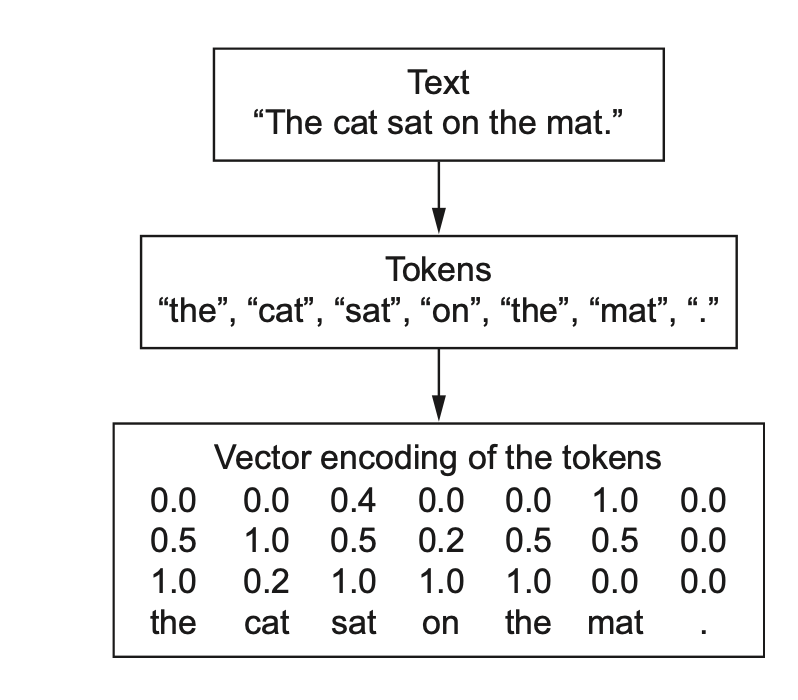
\includegraphics[width=0.4\textwidth]{images/sentence_to_embedding}
    \caption[Embedding Beispiel]{Beispiel für ein Embedding von einem Satz zu Vektoren.}
    \label{fig:sentence_to_embedding}
\end{figure}

Die Vektoren können jetzt in ein Neuronales Netzwerk, das meistens die Transformer-Architektur verwendet, gefüttert werden.
Das Ergebnis besteht aus den Wahrscheinlichkeiten für alle der möglichen nächsten Token.

Im letzten Schritt muss ausgewählt werden, welcher Token genutzt werden soll.
Würde hier immer nur der wahrscheinlichste Token gewählt, würde man nur Texte generieren, die das LLM während des Trainings bekommen hat.
Um einen neuen Text zu generieren werden also zufällig weniger wahrscheinliche Tokens ausgewählt.
Dieser Prozess führt zu dem, was als Halluzinationen bekannt ist.
Es ist ein fester Bestandteil der LLM-Architektur~\cite{fraunhofer_iese2025}.

Mit dem Wissen, wie LLMs funktionieren, kann nun betrachtet werden, wie RAGs funktionieren, wie LLMs mit RAGs kombiniert werden und welche Vorteile RAGs haben.

\section{Funktionsweise von RAGs}

Bei einem Rag kommt das Wissen für die Antwort nicht nur aus dem LLM selbst sondern auch aus angebundenen Quellen.
Diese angebundenen Quellen können Dokumentensammlungen, Datenbanken, Wissensgraphen (Knowledge Graph) oder andere Suchquellen wie eine Internetsuche sein~\cite{honroth2024retrieval}.

\begin{figure}[ht!]
    \centering
    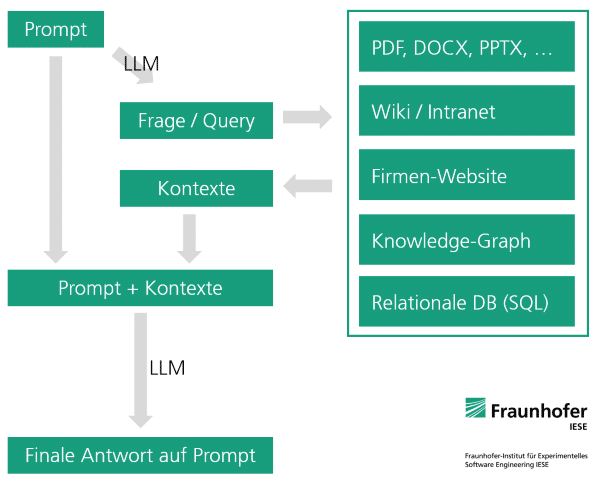
\includegraphics[width=0.8\textwidth]{retrieval_augmented_generation_RAG_600px.png}
    \caption[Struktur eines RAGs]{Struktur eines RAGs, Quelle: \cite{honroth2024retrieval}}
    \label{fig:Rag_Structure}
\end{figure}

Die Abbildung~\ref{fig:Rag_Structure} zeigt den Ablauf für eine Anfrage an ein RAG.
\begin{enumerate}
    \item Im ersten Schritt wird ein Prompt an das LLM gesendet.
    Dieser Prompt besteht aus der Frage des Nutzers, aber auch weiteren Details, wie einer Persona, deren Perspektive das LLM einnehmen soll.
    \item Das LLM kann dann mittels dieses Prompts eine Anfrage generieren, um für diesen Prompt relevante Dokumente zu suchen.
    \item Diese Anfrage gibt dann im optimalen Fall die benötigten Dokumente für die Beantwortung des Prompts zurück.
    Der Schritt des Abfragens relevanter Dokumente wird Retrival genannt.
    Die gefundenen Dokumente werden Kontext genannt.
    \item Der Original Prompt zusammen mit dem abgefragten Kontext wird nun einem LLM zur Verfügung gestellt, um den kontextabhängigen Prompt zu beantworten.
\end{enumerate}
\subsection{Vorteile von RAGs}
Bei der Wissensabfrage durch LLMs zeigen sich unter anderem folgende Schwachstellen:
\begin{description}
    \item [\textbf{Aktualität:}] LLMs kennen nur die verwendeten Trainingsdaten. Es fehl also häufig wissen der letzten Jahre.
    \item [\textbf{Unbalancierte Trainingsdaten:}] Im Trainingsset für die LLMs selten vorkommendes Wissen können LLMs schlecht lernen. \cite{gao2023rtre,2022arXiv221108411K}
    \item [\textbf{Vertraulichkeit:}]Nicht öffentliche Dokumente sind nicht im Trainingsset und daher können LLMs keine Fragen zu nicht öffentlichen Daten beantworten.
\end{description}

Die Nutzung eines RAGs ist eine von drei häufig verwendeten Möglichkeiten, um ein LLM zu verbessern.
Die anderen beiden Möglichkeiten sind Finetuning und die Verwendung eines LLMs mit einem großen Kontextfenster.
Das Finetuning beschreibt das weitere Trainieren eines Modells mit weitere Trainingsdaten.
Die Größe des Kontextfensters beschreibt die Menge an Text, gemessen in Tokens, die das LLM gleichzeitig berücksichtigen kann.
RAGs haben gegenüber dem Finetuning und der Nutzung eines LLMs mit großem Kontextfenster entscheidende Vorteile.\\
ChatGPT-4.1 erreicht inzwischen ein Kontext Window Größe von 1,047,576 Tokens, bei GPT-3.5-Turbo sind es 16,385~\cite{openai_gpt_4_vision}.
Gemini unterstützt ebenfalls bis zu 1 Million Tokens, wobei Google, der Besitzer von Gemini, angibt, dass sie erfolgreich 10 Millionen Token Context Windows getestet haben \cite{google_gemini_next_generation_model}.

\subsection{Faktoren für den Einsatz von RAGs}
Es gibt einige Faktoren, welche die Entscheidung beeinflussen können, ob ein RAG besser für den betrieblichen Ablauf geeignet ist.
Dazu gehören z. B. die Kompetenz der Betreiber des RAGs, die Art der Daten und die finanziellen Möglichkeiten des Unternehmens.


\subsubsection{Kompetenz des Betreibers}
Für das Finetuning von LLMs ist technisches Wissen notwendig, um die Themen Natural Language Processing (NLP), Deep Learning, Modellkonfiguration, Datenaufbereitung und Evaluierung anzuwenden.
Der gesamte Prozess des Finetunings ist technisch anspruchsvoll, erfordert das Kuratieren der neuen Trainingsdaten und ist zudem durch die benötigte Hardware teuer.
Zudem ist das betreiben der Hardware teuer da sie einen hohen Stromverbrauch hat.

Das Benutzen eines LLMs benötigt die geringste Informatische Kompetenz des Anwender, da hier das LLM unverändert bleibt.
Hier werden einfach die Daten inklusive der Frage an das LLM gesendet.
Entscheidend ist allerdings das Erstellen zielführender Prompts, dies benötigt Erfahrung.

Während das LLM in einem RAG auch unverändert bleibt, wird es in ein System mit mehreren Komponenten eingebunden.
Hier ist ein allgemeines Verständnis von LLMs und effektiven Methoden für den Retrieval Teil des RAGs notwendig.
Zudem müssen hier manuell für jedes Dateiformat (E-Mail, PDF etc.) Anbindungen erstellt werden. Sollte ein seltener oder proprietärer Datentyp verwendet werden, muss hier eventuell eigens eine Anbindung entwickelt werden.
\subsubsection{Aktualisierung der Datenbasis}
Sollten die Daten dynamisch sein, wie E-Mails, ist das RAG vermutlich die vorzuziehende Lösung. Dies liegt an den Eigenschaften der schnellen und kontinuierlichen Aktualisierung der Daten.
Wie oben erläutert, kann es jedoch sein, dass es schlechte oder keine Unterstützung von selten verwendeten Dateiformaten gibt.

Der Prozess des Finetunings erstellt hingegen eine Momentaufnahme, die ein erneutes Training erfordert.
Beim Finetuning ist es möglich, dass das Modell Muster erkennt und firmeneigene Begriffe verstehen kann. Dies ist ein deutlicher Vorteil gegenüber dem RAG und dem nutzen eines LLMs mit großem Context Window.


\subsubsection{Budget}
Das Finetuning erfordert über einen langen Zeitraum teure Rechenzeit auf Hochleistungs-Graphical-Processing-Units (Hochleistungs-GPUs).
Dabei handelt es sich um spezialisierte Grafikprozessoren, deren Architektur auf die massive parallele Verarbeitung von Daten optimiert ist, was sie für die rechenintensiven Operationen des Machine Learnings, insbesondere neuronale Netze, unerlässlich macht.
Zudem ist die Qualität der Daten entscheidend; ohne das vorherige Filtern der Daten durch Menschen ist dieser Prozess aktuell nicht möglich. Sollten sich die Daten als unzureichend erweisen, ist die gesamte Rechenzeit verschwendet.
Das RAG verursacht dagegen zusätzliche Kosten durch das Speichern der Daten in einer Vektordatenbank.
Die wohl kostenintensivste Methode ist die Nutzung eines LLMs mit einem großen Kontextfenster.


\section{Objektive Beurteilung von RAGs}
Je mehr Daten einem RAG zur Verfügung stehen, desto aufwendiger ist es, die Qualität des RAGs zu beurteilen.
Eine Beurteilung durch Menschen müsste bei Anpassungen am RAG oder Änderungen an den Daten neu durchgeführt werden.

Tools wie RAGAS, die bereits eine automatisierte Bewertung implementieren, nutzten bei diesem Prozess unter anderem LLMs.
Diese Tools generieren aus den ihnen gegebenen Daten Fragebögen, die zu einer Frage eine beispielhafte Antwort und die genutzten Stellen aus den vorher gegebenen Dokumenten beinhalten.
Sollten nach diesem automatisierten Test die gewünschten Ergebnisse nicht erreicht werden, kann beispielsweise die Veröffentlichung blockiert werden.

Sowohl menschliche Bewertungen als auch je nach Vorgaben die eventuell subjektive Bewertung durch LLMs sind nicht objektiv.
Anhand mehrerer Techniken kann versucht werden, die Bewertung mithilfe von LLMs zu objektivieren. Die Metriken, welche RAGAS nutzt, versuchen z.B. die Anzahl der genannten Fakten aus den Antworten zu extrahieren, um so mit Zahlen arbeiten zu können.

\section{Softwaretechnische Fragestellungen}

In dem Artikel \textit{RAG in der Praxis – Generierung synthetischer Testdatensätze} untersucht Panic~\cite{pixion2024rag} die Testset-Generierung mithilfe von RAGAS. Es treten bei 17 \% der generierten Fragen Fehler beim Generieren der Testfragen auf.
Dies hat vielfältige Gründe, die von nicht verwertbaren Antworten des LLMs bis zu Verbindungsproblemen oder dem Erreichen des Limits der maximalen Anfragen an APIs reichen.

Auch bei der Bewertung von Antworten können sich ungewollte und bisher noch ungeahnte Biases einschleichen. In dem Paper \enquote{Large Language Models are not Fair Evaluators}~\cite{wang-etal-2024-large-language-models-fair} von Wang et al. wird gezeigt, dass, wenn ein LLM eine von zwei gegebenen Antworten aussuchen müsste, die erste bevorzugt wurde, selbst wenn die gleiche Frage mit einer anderen Reihenfolge gestellt wurde.
RAGAS vergleicht keine Antworten miteinander, und daher ist dieser Bias kein direktes Problem für die verwendeten Metriken. Was jedoch einen Einfluss auf die Bewertung von Antworten haben kann, ist der Bias zu gewissen Nummern.
Wie in~\cite{2024arXiv241203605S} von Shaikh et al. beschrieben, bevorzugen LLMs bei der Bewertung lieber Zahlen, welche Vielfache von 5 und 10 sind.

Auch die allgemeine stochastische Natur von LLMs spielt eine Rolle, da bei der gleichen Anfrage unterschiedliche Antworten und somit auch Bewertungen zurückgegeben werden.
Wie groß diese Abweichungen sind, wird in Abschnitt~\ref{subsec:zuverlassigkeit-von-metriken} kurz untersucht.

Wie in dem Paper \enquote{Gemini 1.5: Unlocking multimodal understanding across millions of tokens of context} vom Gemini Team \cite{gemini2024v15} beschrieben, stellt Gemini 1.5 einen bedeutenden Fortschritt in der multimodalen Verarbeitung großer Kontextfenster dar. Das wirft auch die Frage auf, ob RAGs nicht irrelevant sein könnten und durch LLMs mit großen Kontextfenstern abgelöst werden.
Es gibt einige Gründe, die dagegen sprechen: LLMs mit größeren Kontextfenstern werden immer langsamer und teurer; die genauen Kosten sind abzuwarten. Jedes Mal alle Daten in den Kontext zu laden, besonders wenn dies über das Internet geschieht, ist eine weitere Hürde. LLMs fällt es auch schwer, bei zu vielen Informationen noch die relevanten zu finden, was zu schlechteren Antworten führen kann.
Diese Faktoren lassen darauf schließen, dass RAGs, die nicht nur eine einfache Suche nutzen, noch länger relevant bleiben.

Inzwischen werden spezielle LLMs wie Pleias-RAG~\cite{huggingface_pleias_rag_1b} entwickelt.
Diese wurde mittels Finetuning verbessert, um Speziell Aufgaben wie das Suchen und das Zusammenfassen von Dokumenten selbst mit weniger Parametern gut zu können.

% Pitfalls in LLM Assisted Evaluation https://medium.aiplanet.com/evaluate-rag-pipeline-using-ragas-fbdd8dd466c1

\section{Rechtliche Fragestellungen}
\label{sec:rechtliche-fragestellungen}

Am 01.08.2024 trat die \\
\enquote{\textit{VERORDNUNG (EU) 2024/1689 DES EUROPÄISCHEN PARLAMENTS UND DES RATES vom 13. Juni 2024 zur Festlegung harmonisierter Vorschriften für künstliche Intelligenz und zur Änderung der Verordnungen (EG) Nr. 300/2008, (EU) Nr. 167/2013, (EU) Nr. 168/2013, (EU) 2018/858, (EU) 2018/1139 und (EU) 2019/2144 sowie der Richtlinien 2014/90/EU, (EU) 2016/797 und (EU) 2020/1828 (Verordnung über künstliche Intelligenz)}} (KI-VO)~\cite{european_commission_ai_act}\\
in Kraft.
Die Verordnung setzt Regelungen und Maßstäbe für die Verwendung von KI.
RAGs sind gemäß Artikel 3 Nr. 1 in Verbindung mit Artikel 51 KI-VO KI-Systeme~\cite{Martini2024KIVO} und fallen damit in den Anwendungsbereich der KI-VO.
Bei der Nutzung oder Bereitstellung von LLMs muss die KI-VO berücksichtigt werden.
Die Nutzer*innen der RAGs müssen sich der aus der KI-VO ergebenden Pflichten bewusst sein.\\
Ebenso gilt es, bei Anbindung firmeninterner Dokumente die\\
\enquote{\textit{Verordnung (EU) 2016/679 des Europäischen Parlaments und des Rates vom 27. April 2016 zum Schutz natürlicher Personen bei der Verarbeitung personenbezogener Daten, zum freien Datenverkehr und zur Aufhebung der Richtlinie 95/46/EG (Datenschutz-Grundverordnung)}} (DS-GVO) zu beachten.
Die DS-GVO regelt den Umgang mit personenbezogenen Daten, die in solchen firmeninternen Dokumenten enthalten sein könnten.

\section{Konkretisierung der Experimente}

\subsection{Dokumentenverarbeitung}
\begin{table}[htbp]
    \centering
    \begin{tabular}{|c|c|c|c|}
        \hline
        \textbf{Embedding-Modell} & \textbf{10} & \textbf{100} & \textbf{1000} \\
        \hline
        openai/text-embedding-3-large & X & X & X \\
        ollama/nomic-embed-text       & X & X & X \\
        \hline
    \end{tabular}
    \caption{Kombinationen aus Dokumentanzahl und Embedding-Modell für die Experimente (X = Kombination wird getestet)}
    \label{tab:dokument-erstellung}
\end{table}

Für die Experimente werden folgende Dokumentmengen und -typen verwendet:

\begin{itemize}
    \item Für die Experimente mit \textbf{10 Dokumenten} werden existierende Dokumente ausgewählt.
    \item Für die Experimente mit \textbf{100} und \textbf{1000 Dokumenten} müssen zusätzliche Dokumente generiert werden, vorzugsweise mit einem LLM.
\end{itemize}

\noindent
In allen Versuchen werden Dateien der folgenden Typen verwendet:

\begin{itemize}
    \item PDF (.pdf)
    \item Klartext (.txt)
    \item Word-Dokumente (.docx, .doc)
    \item Excel-Tabellen (.xlsx, .xls)
    \item CSV-Dateien (.csv)
    \item E-Mails (.eml)
    \item PowerPoint-Präsentationen (.pptx, .ppt)
\end{itemize}

\subsection{Testset-Generierung}
Die Question Synthesizers bleiben in allen Experimenten gleich.  
Weitere Informationen: \url{https://docs.ragas.io/en/stable/concepts/test_data_generation/rag/}

\begin{itemize}
    \item \textbf{SingleHopSpecificQuerySynthesizer} (Gewichtung: 0{,}5)
    \item \textbf{MultiHopAbstractQuerySynthesizer} (Gewichtung: 0{,}25)
    \item \textbf{MultiHopSpecificQuerySynthesizer} (Gewichtung: 0{,}25)
\end{itemize}

Um die optimale Anzahl an Fragen pro Testset zu untersuchen, werden folgende Kombinationen generiert:

\begin{table}[htbp]
    \centering
    \begin{tabular}{|c|c|c|}
        \hline
        \textbf{Dokumentanzahl} & \textbf{Anzahl Fragen pro Testset} & \textbf{Anzahl Testsets pro Modell} \\
        \hline
        10   & 15, 30    & 2 \\
        100  & 50, 100   & 2 \\
        1000 & 150, 300  & 2 \\
        \hline
        \multicolumn{2}{|c|}{\textbf{Summe Testsets pro Modell}} & 6 \\
        \hline
    \end{tabular}
    \caption{Kombinationen aus Dokumentanzahl und Testset-Größe}
\end{table}

\subsection{Bewertung}
Um die Robustheit und Übertragbarkeit der Bewertungsergebnisse zu erhöhen, werden alle Kombinationen aus Embedding-Modell und Bewertungsmodell getestet. Das bedeutet, dass für jedes Testset sowohl openai/text-embedding-3-large als auch ollama/nomic-embed-text als Embedding-Modell verwendet werden und die Bewertung jeweils mit GPT-4 sowie Deepseek-R1 (ollama/deepseek-r1:7b) erfolgt. Insgesamt ergeben sich so 24 Experimente (2 Embeddings × 2 Bewerter × 6 Testset-Varianten).

\begin{table}[htbp]
    \centering
    \begin{tabular}{|c|c|c|c|c|c|c|}
        \hline
        \textbf{Experiment} & \textbf{Embedding} & \textbf{Dokumente} & \textbf{Fragen} & \textbf{Bewerter} & \textbf{Richter} & \textbf{Wdh.} \\
        \hline
        1  & OAI-E & 10   & 15  & GPT-4 & GPT-4 & 1 \\
        2  & OAI-E & 10   & 30  & GPT-4 & GPT-4 & 4 \\
        3  & OAI-E & 100  & 50  & GPT-4 & GPT-4 & 1 \\
        4  & OAI-E & 100  & 100 & GPT-4 & GPT-4 & 4 \\
        5  & OAI-E & 1000 & 150 & GPT-4 & GPT-4 & 1 \\
        6  & OAI-E & 1000 & 300 & GPT-4 & GPT-4 & 1 \\
        \hline
        7  & OAI-E & 10   & 15  & DSK-R & DSK-R & 1 \\
        8  & OAI-E & 10   & 30  & DSK-R & DSK-R & 1 \\
        9  & OAI-E & 100  & 50  & DSK-R & DSK-R & 1 \\
        10 & OAI-E & 100  & 100 & DSK-R & DSK-R & 1 \\
        11 & OAI-E & 1000 & 150 & DSK-R & DSK-R & 1 \\
        12 & OAI-E & 1000 & 300 & DSK-R & DSK-R & 1 \\
        \hline
        13 & OLL-E & 10   & 15  & GPT-4 & GPT-4 & 1 \\
        14 & OLL-E & 10   & 30  & GPT-4 & GPT-4 & 1 \\
        15 & OLL-E & 100  & 50  & GPT-4 & GPT-4 & 1 \\
        16 & OLL-E & 100  & 100 & GPT-4 & GPT-4 & 1 \\
        17 & OLL-E & 1000 & 150 & GPT-4 & GPT-4 & 1 \\
        18 & OLL-E & 1000 & 300 & GPT-4 & GPT-4 & 1 \\
        \hline
        19 & OLL-E & 10   & 15  & DSK-R & DSK-R & 1 \\
        20 & OLL-E & 10   & 30  & DSK-R & DSK-R & 4 \\
        21 & OLL-E & 100  & 50  & DSK-R & DSK-R & 1 \\
        22 & OLL-E & 100  & 100 & DSK-R & DSK-R & 1 \\
        23 & OLL-E & 1000 & 150 & DSK-R & DSK-R & 1 \\
        24 & OLL-E & 1000 & 300 & DSK-R & DSK-R & 1 \\
        \hline
    \end{tabular}
    \caption{Übersicht aller 24 zu generierenden Bewertungsberichte mit Abkürzungen und Wiederholungen}
    \label{tab:bewertungsberichte}
\end{table}

\noindent
\textbf{Verwendete Abkürzungen in der Tabelle:}
\begin{itemize}
    \item \textbf{OAI-E} = openai/text-embedding-3-large
    \item \textbf{OLL-E} = ollama/nomic-embed-text
    \item \textbf{GPT-4} = openai/gpt-4
    \item \textbf{DSK-R} = ollama/deepseek-r1:7b
\end{itemize} 
\section{Experimentplan}

Um systematisch zu bewerten, ob RAG-Bewertungstools für den Einsatz in kleineren Unternehmen bereit sind, ist ein umfassender experimenteller Ansatz erforderlich. Der folgende Experimentplan skizziert die wichtigsten Variablen, die Methodik und die Bewertungskriterien.

\subsection{Forschungsfragen}

Das Experiment wird die folgenden zentralen Forschungsfragen behandeln:

\begin{enumerate}
    \item Sind aktuelle RAG-Bewertungsframeworks in Bezug auf Kosten, Komplexität und Ressourcenanforderungen für den Einsatz in kleinen Unternehmen geeignet?
    \item Wie beeinflussen verschiedene Dokumenttypen und Datenvolumina die Qualität von Abruf und Generierung?
    \item Wie zuverlässig und konsistent sind die verfügbaren Bewertungsmetriken zur Beurteilung der RAG-Leistung?
    \item Was ist das optimale Gleichgewicht zwischen Kosten, Leistung und Implementierungskomplexität für jeden Anwendungsfall in kleinen Unternehmen?
\end{enumerate}

\subsection{Experimentelle Variablen}

\subsubsection{Dokumenttypen}
Verschiedene Dokumentformate werden getestet, um die Vielseitigkeit des Systems zu bewerten:
\begin{itemize}
    \item Klartext (.txt)
    \item PDF-Dokumente mit Text, Tabellen und Bildern
    \item HTML-Inhalte von Webseiten
    \item Microsoft Office-Dokumente (.docx, .xlsx)
    \item JSON und strukturierte Datenformate
\end{itemize}

\subsubsection{Datenvolumen}
Die Skalierbarkeit des Systems wird mit unterschiedlichen Datenmengen getestet:
\begin{itemize}
    \item Klein (10-50 Dokumente, ~100 Seiten) dies könnte pro Anwendungsfall eingerichtet und nach dem Experiment verworfen werden
    \item Mittel (100-500 Dokumente, ~1.000 Seiten) dies könnte pro Benutzer eingerichtet werden und im Laufe der Zeit wachsen
    \item Groß (1.000+ Dokumente, ~10.000 Seiten) dies könnte unternehmensweit eingerichtet werden und im Laufe der Zeit wachsen
\end{itemize}

\subsubsection{Modelle zur Bewertung}
Mehrere Modelle werden bewertet, die verschiedene Kostenschichten und Fähigkeiten repräsentieren.\
Hierbei ist es wichtig zu überlegen, welche Optionen für kleine Unternehmen gültige Anwendungsfälle sind.
Open-Source-Modelle (z.B. Llama 2, Mistral 7B, Deepseek R1) bieten eine Vielzahl von Vorteilen, wie die Möglichkeit, sie zu modifizieren und mehr Kontrolle über die Daten zu haben, was rechtliche Vorteile bietet, aber auch Nachteile. Die Fähigkeit, sie selbst zu hosten, kann ein Plus, aber auch ein Minus sein, je nach Art des Unternehmens.\
Mittelklasse-API-Modelle (z.B. Claude Haiku, GPT-3.5 Turbo) sind günstiger als die Hochleistungsmodelle und bieten dennoch eine gute Leistung. Da sie nicht Open Source sind, bieten sie weniger Kontrolle über die Daten und das Modell selbst, manchmal muss man mehr für private Instanzen zahlen.\
Hochleistungsmodelle (z.B. GPT-4, Claude 3 Opus) sind die teuerste Option, bieten aber auch die beste Leistung, sowohl in Bezug auf Geschwindigkeit als auch auf die Qualität der generierten Antworten. Sie haben ähnliche Vor- und Nachteile wie die Mittelklasse-API-Modelle. \
Aus rechtlicher Sicht sind die Hochleistungsmodelle die sicherste Option, da sie bestimmte Dokumentationen veröffentlichen und rechtliche Garantien bieten müssen.
% TODO: artikel 53 und Anhang 12 und 13
% TODO: erklären

\subsubsection{Bewertungsmetriken}
Während des Experiments werden neben der menschlichen Bewertung zwei Frameworks zur Bewertung verwendet.
Giskard und RAGAS werden die später beschriebenen Metriken generieren, die später verglichen und bewertet werden können.
Die menschliche Bewertung wird als subjektives Maß verwendet, um die Ergebnisse der anderen beiden zu vergleichen.

\subsection{Kosten- und Zeitanalyse}
Ob wir dies tun wollen, ist noch nicht klar, RAGAS bietet Kostenberechnung an, aber ich habe es mir noch nicht angesehen.

\subsection{Experimentelles Protokoll}

\begin{enumerate}
    \item \textbf{Dokumentensammlung und -vorbereitung}
    Sammeln Sie Dokumente in allen oben genannten Zielformaten.
    
    \item \textbf{Testset-Generierung}
    Generieren Sie verschiedene Fragetypen (faktisch, inferentiell, vergleichend) und erstellen Sie Referenzantworten zur Bewertung.
    Dies geschieht automatisch durch das RAGAS-Framework.
    Validieren Sie das Testset manuell auf Qualität und Abdeckung, dies wird an einer Reihe zufälliger Proben durchgeführt.
    
    
    \item \textbf{Systemkonfiguration}
    Konfigurieren Sie Einbettungsmodelle und Parameter, richten Sie Vektorspeicher mit konsistenten Einstellungen ein und setzen Sie Bewertungsframeworks ein.
    
    \item \textbf{Durchführung der Bewertung}
    Da wir die hochgeladenen Dateien, die generierten Dokumente und das Testset wiederverwenden können, werden diese zuerst erstellt.
    Dann wird die Bewertungspipeline ausgeführt und die Ergebnisse werden aufgezeichnet.
    
    \item \textbf{Analyse und Berichterstattung}
    Vergleichende Analyse über alle Variablen hinweg, Kosten-Nutzen-Analyse für geschäftliche Entscheidungsfindung und Empfehlungen für optimale Konfigurationen.
\end{enumerate}

\subsection{Bewertungskriterien für die Geschäftsfähigkeit}

Die endgültige Bewertung wird RAG-Systeme in diesen Dimensionen bewerten:
\begin{itemize}
    \item \textbf{Implementierungskomplexität}: Wie schwierig ist die Einrichtung und Wartung?
    \item \textbf{Kostenvorhersehbarkeit}: Sind die Kosten stabil und vorhersehbar?
    \item \textbf{Leistungszuverlässigkeit}: Leistet das System konsistent?
    \item \textbf{Skalierbarkeit}: Wie gut bewältigt das System wachsende Datenanforderungen?
    %\item \textbf{Integrationspotenzial}: Kann es mit bestehenden Geschäftssystemen verbunden werden?
    %\item \textbf{Gesamtkosten des Eigentums}: Was sind die vollständigen Kosten über die Zeit?
\end{itemize}

Dieser experimentelle Ansatz bietet einen umfassenden Rahmen, um zu bewerten, ob aktuelle RAG-Bewertungstools ausreichend ausgereift für die Einführung in kleinen Unternehmen sind, mit klaren Anleitungen zu optimalen Konfigurationen und Implementierungsstrategien. 
\section{RAG-Bewertungsprozess}

Das Flussdiagramm veranschaulicht die drei Hauptphasen des RAG-Bewertungsprozesses:

\begin{enumerate}
    \item \textbf{Dokumentenverarbeitung}
    \begin{itemize}
        \item Dokumente werden geladen und in Abschnitte unterteilt
        \item Textabschnitte werden eingebettet
        \item Eingebettete Vektoren werden in ChromaDB gespeichert
    \end{itemize}
    
    \item \textbf{Erstellung des Testsets}
    \begin{itemize}
        \item Verwendet LLM zur Generierung von Fragen
        \item Erstellt Testsets mit Fragen und Referenzantworten
    \end{itemize}
    
    \item \textbf{Bewertungsprozess}
    \begin{itemize}
        \item Verwendet das generierte Testset
        \item Ruft Kontext aus ChromaDB ab
        \item Bewertet Modellantworten mit LLM als Richter
        \item Generiert umfassende Bewertungsberichte
    \end{itemize}
\end{enumerate}

\begin{figure}[htbp]
    \centering
    \resizebox{\textwidth}{!}{
    \begin{tikzpicture}[
        node distance=1.8cm and 1.5cm,
        model/.style={rectangle, draw, fill=pink!20, text width=3cm, text centered, minimum height=1cm, rounded corners=3pt},
        storage/.style={rectangle, draw, fill=blue!20, text width=3cm, text centered, minimum height=1cm, rounded corners=3pt},
        process/.style={rectangle, draw, fill=green!20, text width=3cm, text centered, minimum height=1cm, rounded corners=3pt},
        data/.style={rectangle, draw, fill=red!20, text width=3cm, text centered, minimum height=1cm, rounded corners=3pt},
        arrow/.style={thick,->,>=stealth},
        stage_label/.style={font=\bfseries, text width=3.5cm, text centered, node distance=0.8cm}
    ]
        % Stage 1: Datenverarbeitung
        \node[data] (doc) {Dokumentensammlung};
        \node[stage_label] (stage1_label) [above=of doc] {Phase 1: Datenverarbeitung};
        \node[process] (dl) [below=of doc] {Dokumentenlader};
        \node[data] (chunks) [below=of dl] {\textbf{Textabschnitte}};
        \node[model] (emb1) [below=of chunks, xshift=-2cm] {Einbettungsmodell für die Dokumentenverarbeitung};
        \node[storage] (vstore) [below=of chunks, xshift=2cm] {Vektorspeicher};
        \node[storage] (chroma) [below=of vstore] {ChromaDB-Sammlung};

        % Stage 2: Testset-Erstellung
        \node[process] (tsgen) [right=4.5cm of doc, yshift=-1cm] {Testset-Generator};
        \node[stage_label] (stage2_label) [above=of tsgen] {Phase 2: Testset-Erstellung};
        \node[model] (llm1) [above left=0.8cm and 0.4cm of tsgen] {LLM für die Testset-Generierung};
        \node[model] (emb2) [below left=0.8cm and 0.4cm of tsgen] {Einbettungsmodell für die Testset-Generierung};
        \node[data] (testset) [below=of tsgen] {Testset};

        % Stage 3: RAG-Bewertung
        \node[process] (eval) [right=4.5cm of tsgen, yshift=1cm] {Bewertung};
        \node[stage_label] (stage3_label) [above=of eval] {Phase 3: RAG-Bewertung};
        \node[model] (llm2) [above left=0.8cm and 0.4cm of eval] {\textbf{Zu bewertendes Modell}};
        \node[model] (llm3) [below left=0.8cm and 0.4cm of eval] {LLM-Modell als Richter};    
        \node[data] (report) [below=of eval] {Bewertungsbericht};
        \node[storage] (repfile) [below=of report] {Berichtsdateien};

        % Verbindungen
        % Dokumentenverarbeitungsfluss
        \draw[arrow] (doc) -- (dl);
        \draw[arrow] (dl) -- (chunks);
        \draw[arrow] (chunks) -| (emb1);
        \draw[arrow] (chunks) -| (vstore);
        \draw[arrow] (emb1) -- (vstore);
        \draw[arrow] (vstore) -- (chroma);

        % Testset-Generierungsfluss
        \draw[arrow] (doc) -- (tsgen);
        \draw[arrow] (llm1) -- (tsgen);
        \draw[arrow] (emb2) -- (tsgen);
        \draw[arrow] (tsgen) -- (testset);

        % Bewertungsfluss
        \draw[arrow] (testset.north east) to[bend left=15] (eval.west);
        \draw[arrow] (chroma.east) -| (eval.west);
        \draw[arrow] (llm2) -- (eval);
        \draw[arrow] (llm3) -- (eval);
        \draw[arrow] (eval) -- (report);
        \draw[arrow] (report) -- (repfile);
    \end{tikzpicture}
    }
    \caption{Flussdiagramm des RAG-Bewertungsprozesses, das die Interaktion zwischen verschiedenen Komponenten und Modellen zeigt. Spezifische Modellnamen (z.B. gpt-4-turbo, text-embedding-3-large) sind im Haupttext beschrieben.}
    \label{fig:rag-flow}
\end{figure}

% Farblegende für das Flussdiagramm
\begin{center}
\begin{minipage}{0.85\textwidth}
\textbf{Legende für Flussdiagrammfarben:}
\begin{itemize}
    \item \colorbox{pink!20}{\strut\hspace{1.5em}} \textbf{Modell}: (z.B. LLMs, Einbettungsmodelle)
    \item \colorbox{blue!20}{\strut\hspace{1.5em}} \textbf{Speicher}: (z.B. Vektorspeicher, ChromaDB)
    \item \colorbox{green!20}{\strut\hspace{1.5em}} \textbf{Prozess}: (z.B. Dokumentenlader, Bewertung)
    \item \colorbox{red!20}{\strut\hspace{1.5em}} \textbf{Daten}: (z.B. Dokumentensammlung, Testset, Bericht)
\end{itemize}
\end{minipage}
\end{center}

Das Diagramm hebt hervor, wie bestimmte Komponenten, wie LLM, für verschiedene Zwecke wiederverwendet werden, während separate Einbettungsmodelle für spezifische Aufgaben beibehalten werden. Dieser modulare Ansatz ermöglicht flexible Experimente mit verschiedenen Modellen und Konfigurationen, während ein konsistentes Bewertungsframework beibehalten wird. 
\chapter{Metrics}

\label{chap:formal}
In diesem Kapitel geht es um die verschiedenen Metriken, die für die Bewertung von RAG Evaluations Tools verwendet werden können.
Metriken sind das Herzstück der Bewertung von RAGs, da sie die Qualität des RAGs bewerten und somit die Entwicklung und den Fortschritt des RAGs messen.


\section{Retrieval Augmented Generation}
Diese Metriken basieren auf Faktenextraktion mithilfe welcher sich dann Scores berechnen lassen.
Für die extraktion der Fakten wird häufig ein LLM verwendet welcher als Richter fungiert.


\subsection{Context Precision}
\begin{quote}
Die Kontextpräzision ist eine Metrik, die den Anteil relevanter Textabschnitte in den abgerufenen Kontexten misst.
Sie wird als Mittelwert der Präzision@k für jeden Textabschnitt im Kontext berechnet.
Die Präzision@k ist das Verhältnis der Anzahl relevanter Textabschnitte auf Rang k zur Gesamtanzahl der Textabschnitte auf Rang k.
(eigene Übersetzung nach \cite{ragas_context_precision})
\end{quote}
Diese Metrik ist für uns als Qualitätskontrolle wichtig da sie uns sagt, ob es Probleme beim testen mit dem Vectorstore gibt.

\subsection{Context Recall}
\begin{quote}
Context Recall misst, wie viele der relevanten Dokumente (oder Informationsstücke) erfolgreich abgerufen wurden.
Es konzentriert sich darauf, keine wichtigen Ergebnisse zu verpassen.
Ein höherer Recall bedeutet, dass weniger relevante Dokumente ausgelassen wurden.
Kurz gesagt geht es beim Recall darum, nichts Wichtiges zu übersehen.
(eigene Übersetzung nach \cite{ragas_context_recall})
\end{quote}

Wenn es eine guten guten Context Precision Score gibt dann lässt sich hier gut bewerten ob das LLM in der Lage ist die relevanten Informationen in dem kontext zu finden.
Da dies ein wichtiger Aspekt eines guten RAGs ist wird diese Metrik im Rahmen dieser Arbeit betrachtet.

\subsection{Context Entities Recall}
In deisem Kontext ist eine Entity eine Informationseinheit, die im Kontext vorkommt.
Dies könnte z.B. ein Name, ein Ort, ein Datum oder eine andere Informationseinheit sein.

\begin{quote}
Die ContextEntityRecall-Metrik misst den Recall des abgerufenen Kontexts, basierend auf der Anzahl der Entitäten, die sowohl in der Referenz als auch im abgerufenen Kontext vorkommen, relativ zur Gesamtanzahl der Entitäten in der Referenz.\\
Einfach ausgedrückt misst sie, welcher Anteil der Entitäten aus der Referenz im abgerufenen Kontext wiedergefunden wird.\\
(eigene Übersetzung nach \cite{ragas_context_entities_recall})
\end{quote}
Diese Metrik wird Teil dieser arbeit sein da sie in gewissen nutzungsfällen, wie z.B. stark faktuale Fragen, eine gute Bewertung liefern kann.

\subsection{Noise Sensitivity}
\begin{quote}
NoiseSensitivity misst, wie häufig ein System Fehler macht, indem es falsche Antworten gibt, wenn entweder relevante oder irrelevante abgerufene Dokumente verwendet werden.\\
Um die Noise Sensitivity zu bestimmen, wird jede Aussage in der generierten Antwort daraufhin überprüft, ob sie auf der Grundlage der Referenz korrekt ist und ob sie dem relevanten (oder irrelevanten) abgerufenen Kontext zugeordnet werden kann.\\
(eigene Übersetzung nach \cite{ragas_noise_sensitivity})
\end{quote}
Diese Metrik ist eine der wichtigsten Metriken in dieser Arbeit da sie die Richtigkeit der Antworten und damit die Qualität des RAGs bewertet.

\subsection{Response Relevancy}
\begin{quote}
Die ResponseRelevancy-Metrik misst, wie relevant eine Antwort im Bezug auf die Nutzereingabe ist. Höhere Werte zeigen eine bessere Übereinstimmung mit der Nutzereingabe an, während niedrigere Werte vergeben werden, wenn die Antwort unvollständig ist oder redundante Informationen enthält.\\
(eigene Übersetzung nach \cite{ragas_response_relevancy})
\end{quote}

Diese Metrik bildet mit der Noise Sensitivity eine wichtige Grundlage für die Bewertung des RAGs.
Denn selbst wenn die Antworten richtig sind, ist die Bewertung des RAGs nicht gut wenn die Antworten nicht relevant zu der Frage sind.

\subsection{Faithfulness}
\begin{quote}
Die Faithfulness-Metrik misst, wie faktentreu eine Antwort im Vergleich zum abgerufenen Kontext ist.\\

Eine Antwort gilt als faktentreu, wenn alle ihre Aussagen durch den abgerufenen Kontext gestützt werden können.\\

Die Berechnung erfolgt nach folgender Formel:
\begin{align}
  \text{Faithfulness Score} 
    &= \frac{
        \parbox{7cm}{\centering Anzahl der durch den Kontext\\ gestützten Aussagen in der Antwort}
      }{
        \parbox{7cm}{\centering Gesamtanzahl der Aussagen\\ in der Antwort}
      }
  \end{align}

(eigene Übersetzung nach \cite{ragas_faithfulness})
\end{quote}
\subsection{Multimodal Faithfulness/Multimodal Relevance}
Da sich diese Metriken mit mehr als textuellen Daten befassen, werden diese nicht im Rahmen dieser Arbeit betrachtet.


\section{Nvidia Metrics}
Diese Metriken sind subjektiver Art und benutzten wieder eine LLM um die Bewertung zu treffen.
Hier werden einzelnde Scores generiert welche keinen tieferen Einblick in die Bewertung gewähren.

\subsection{Answer Accuracy}
\begin{quote}
Answer Accuracy misst die Übereinstimmung zwischen der Antwort eines Modells und einer Referenz (Ground Truth) für eine gegebene Frage. Dies geschieht über zwei verschiedene "LLM-as-a-judge"-Prompts, die jeweils eine Bewertung (0, 2 oder 4) zurückgeben. Die Metrik wandelt diese Bewertungen in eine Skala von [0,1] um und nimmt dann den Durchschnitt der beiden Bewertungen der Richter.
\\
(eigene Übersetzung nach \cite{ragas_nvidia_metrics})
\end{quote}

Das LLM bewertet die Antwort mit der Referenz und auch die Referenz mit der Antwort.
Hat Vorteile gegenüber der Answer Correctness, da es weniger Aufrufe mit weniger Tokens an LLM braucht.
Es werden im Vergleich zur Answer Correctness auch robustere Bewertungen getroffen, bietet jedoch weniger Einblicke in die Bewertung.
Diese Metrik wird im Rahmen dieser Arbeit betrachtet auch um einen Vergleich zu anderen Metriken zu haben.

\subsection{Context Relevance}
Diese Metrik ist sehr ähnlich zur Context Precision, als Alternative und um einen Vergleich zu haben wird diese im Rahmen dieser Arbeit betrachtet, auch wenn sie keine direkte Aussage über das zu bewertende LLM macht.

\subsection{Response Groundedness}
Wenn die Answer Accuracy eine gute Bewertung liefert, ist die Response Groundedness eine gute Bewertung für die Faktualität der Antwort.
Diese Logik ist ähnlich zur Kombinierung von Context Relevancy und Context Precision.
Hier wird es in den Experimenten interessant zu vergleichen wie diese Metriken zusammenhängen.
\section{Natural Language Comparison}

\subsection{Factual Correctness}
Diese Metriken basieren zu Teilen auf der Wahrheitsmatrix (Confusion matrix), welche die vier Kategorien True Positive, False Positive, False Negative und True Negative definiert.\cite{wikipedia_confusion_matrix}
Aus dieser Matrix lassen sich dann precision, recall und f1 score berechnen.

\begin{quote}
\begin{equation}
  \label{eq:precision}
  \text{Precision} = \frac{\text{True Positives}}{\text{True Positives} + \text{False Positives}}
\end{equation}

\begin{equation}
  \label{eq:recall}
  \text{Recall} = \frac{\text{True Positives}}{\text{True Positives} + \text{False Negatives}}
\end{equation}

\begin{equation}
  \label{eq:f1_score}
  \text{F1 Score} = 2 \cdot \frac{\text{Precision} \cdot \text{Recall}}{\text{Precision} + \text{Recall}}
\end{equation}
\cite{wikipedia_confusion_matrix}
\end{quote}

\subsection{Semantic Similarity}
This metric uses embeddings to calculate the semantic similarity between the answer and the reference. TODO: should this be used?

\section{Non LLM String Similarity}
Wie der Name schon sagt, wird die String Similarity ohne LLM berechnet. Diese Metriken sind relative einfache Metriken und werden im Rahmen dieser Arbeit keine große Rolle spielen, jedoch als Vergleich zu anderen Metriken dienen.
\subsection{BLEU Score}
Misst die Ähnlichkeit zwischen der Antwort und der Referenz. Dabei wird die Wortanzahl der Referenz berücksichtigt und eine entsrechende Bestrafung für zu kurze Antworten eingeführt.
\subsection{ROUGE Score}
Mithilfe von n-gram recall, precision, und dem F1 score wird die Ähnlichkeit zwischen der Antwort und der Referenz berechnet.
\subsection{String Presence}
Eine einfache Metrik um zu sehen, ob die Referenz in der Antwort enthalten ist.
\subsection{Exact Match}
Eine noch einfachere Metrik, die nur prüft ob die Antwort exakt der Referenz entspricht. Diese ist für einzelde Wörter sinnvoll.

\section{General purpose}
Dies sind Metriken welche manuell konfiguriert werden müssen aber eine gute Bewertung der Qualität eines RAGs liefern können.
Die Metriken reichen von einfachen Fragen wie "ist die Antwort schädlich oder hat die Intention des Users verletzt" bis hin zu komplexeren einlend definierten Scrores.
\begin{itemize}
    \item Aspect critic
    \item Simple Criteria Scoring
    \item Rubrics based Scoring
    \item Instance Specific Rubrics Scoring
  \end{itemize}

\section{Andere Metriken}
\subsection{Summarization}
Anzahl der richtig beantworteten Fragen geteilt durch die Anzahl der Fragen. Dies ist eine sehr einfache und oberflächliche Metrik.


\section{Irrelevante Metriken}
\subsection{SQL}
SQL spezifische Metriken welche nicht im Rahmen dieser Arbeit betrachtet werden.

\subsection{Agents or Tool use cases}
Metriken zum bewerten des einsatzes von Agents oder Tools, dies liegt ebenso außerhalb des Themas dieser Arbeit.
https://docs.ragas.io/en/stable/concepts/metrics/
%\chapter{Gestaltung: Textsatz mit \LaTeX}
\label{chap:Textsatz}
%
Mit \LaTeX{} ist es verhältnismäßig einfach, Dokumente zu erstellen, die professionellen Ansprüchen genügen. Ein entscheidender Vorteil ist, dass der Nutzer fast nur den Inhalt beisteuert, während die korrekte äußere Form dann automatisch erzeugt wird. \LaTeX{} basiert auf \TeX{}, das von Donald Knuth entwickelt wurde~\cite{knuth:tex}. Einige weitere Vorteile gegenüber gängiger
Textverarbeitung:
\begin{description}
	\item[Frei/Plattformunabhägig:] Bei \LaTeX{} handelt es sich um freie 
	Software. Es wird kein proprietärer Editor benötigt, um \LaTeX{}-Dokumente
	zu schreiben. Tatsächlich können die Dokumente auf \emph{jedem} Rechner
	mit \emph{jedem} beliebigen Editor bearbeitet werden.
	%
	\item[Reines Textformat:] Der Quelltext~--~die \texttt{tex}-Datei~--~ist
	ein reines Textformat. Dadurch eignen sich \LaTeX{}-Dokumente auch 
	hervorragend zur Versionskontrolle mit beispielsweise git. Dies wiederum
	ermöglicht eine effiziente Zusammenarbeit mehrerer Autor*innen.
	%
	\item[Aufteilen großer Dokumente:] Der Quelltext großer Dokumente, wie 
	beispielsweise von Projektarbeiten, kann auf mehrere Dateien
	aufgeteilt werden. So können beispielsweise mehrere Personen an jeweils
	einem eigenen Kapitel arbeiten. Aufgrund der beiden oberen Punkte wird es 
	auch nicht zu Kompatibilitätsproblemen kommen.
	%
	\item[Trennen von Layout/Inhalt:] Mit \LaTeX{} kann man explizit das
	Layout für das gesamte Dokument festlegen -- oder die verwendete 
	Dokumentklasse kümmert sich implizit darum. Zeitgemäße Textverarbeitung
	bietet mit Formatvorlagen zwar entsprechende Funktionalitäten; aber
	durch den programmatischen Ansatz mit \LaTeX{} kann noch genauer
	Einfluss auf das Layout genommen werden. Anschließend kann die ganze
	Konzentration auf das Schreiben gelegt werden.
	%
	\item[Professionelles Ergebnis:] Ein mit \LaTeX{} erzeugtes Dokument
	schaut professioneller aus, als ein entsprechendes, mit Textverarbeitung
	erzeugtes Dokument. Das gilt vor allem für mathematiklastige Dokumente.
	Aber auch andere Dokumente können von einem einheitlichen 
	Layout, gleichmäßigem Grauwert des Fließtexts, stimmigeren Seitenumbrüchen 
	und hochwertigen Vektorgraphiken profitieren~--~um nur mal einige Punkte zu 
	nennen.
	%
	\item[Vielseitig einsetzbar:] Mit \LaTeX{} können nicht nur 
	\enquote{einfache} Dokumente erzeugt werden. Es existieren unzählige
	Dokumentklassen, die beispielsweise auch das Erstellen von Präsentationen
	oder Postern ermöglichen.
\end{description}
\par
In den folgenden Abschnitten \ref{sec:hood} bis \ref{sec:template} wird auf diverse Aspekte eingegangen, die Sie beim Erstellen Ihres Dokuments berücksichtigen sollten.
%
%
\section{Unter der Haube}
\label{sec:hood}
Sie definieren in Ihren \texttt{TEX}-Dokumenten, was Ihre Inhalte sind (Text mit Gliederung, Bilder, Tabellen, Literaturverweise, \ldots) und wie diese jeweils grob aussehen sollen (z.\,B.\ Platzierung von Abbildungen mittels \emph{Gleitumgebungen}, vgl. \cref{sec:figures}).
\par
Beim Erstellen des endgültigen Dokuments wendet \LaTeX{} \enquote{unter der Haube} eine ganze Menge Regeln an, die festlegen, wie das alles bestmöglich umgesetzt werden kann. Diese Regeln betreffen z.\,B.\ den Anteil von Text und Bildern pro Seite, Abstände innerhalb von Zeilen, aber auch Sonderfälle wie das Vermeiden einzelner Zeilen eines Abschnitts alleine auf einer Seite (sog.\ \enquote{Schusterjungen} oder \enquote{Hurenkinder}).
\par
Im Ergebnis kann es also passieren, dass z.\,B.\ Ihre Abbildungen \enquote{springen}, während Sie an Ihrem Text arbeiten. Das hat im Zweifel alles seine Richtigkeit und kann im Notfall am Ende noch optimiert werden.
\par
In diesem Zusammenhang ist zu vermeiden, in den Gestaltungsprozess einzugreifen, indem z.\,B. manuell Zeilenumbrüche (\comm{newline} oder \comm{\textbackslash}) eingefügt werden oder Abstände. Ausnahmen bitte nur in begründeten Fällen wie in dieser Vorlage bei der Gestaltung des Deckblatts.
\par
Weitere Infos dazu, wie Sie mit dieser Vorlage hier weiterarbeiten können, finden Sie in \cref{sec:template}.
%
%
\section{Überschriften}
\label{sec:headings}
Wir nutzen in dieser Vorlage das Kapitel (\comm{chapter}) als höchste Gliederungsebene. Danach kommen Abschnitte (\comm{section}) und Unterabschnitte (\comm{subsection}). Diese drei Ebenen werden nummeriert und erscheinen im Inhaltsverzeichnis. Falls Sie Ihren Text weiter gliedern wollen, gibt es noch den \comm{paragraph}-Befehl.
\par
Bitte beachten Sie, dass im Text nie zwei Überschriften direkt aufeinander folgen sollten. Nach einer Überschrift kommt immer erst etwas Text (siehe z.\,B.\ die Kapitelanfänge hier auf Seite~\pageref{chap:formal} und Seite~\pageref{chap:Textsatz}). Für weitere Hinweise vgl. \cref{sec:listOfContents}.
%
%
\section{Absätze}
Stellen im Text, an denen ein neuer Absatz beginnen soll, können im Quellcode durch \comm{par} markiert werden. Wie diese Absätze im fertigen Dokument genau aussehen, wird durch den Parameter \comm{parskip} in der Dokumentenklasse bestimmt~--~dazu mehr in \cref{sec:template}. Das ist ein großer Vorteil von \LaTeX{}: Der Stil kann jederzeit für das gesamte Dokument einfach verändert werden.
\par
Hinweis: Sie erhalten das gleiche Verhalten auch, wenn Sie im Quellcode statt des \comm{par}-Befehls eine leere Zeile stehen lassen. Vielleicht gefällt Ihnen das sogar noch besser.
%
%
\section{Silbentrennung}
\label{sec:hyphenation}
Die automatische Silbentrennung in \LaTeX{} funktioniert grundsätzlich gut. Es kann aber immer mal kleinere Probleme und erwünschtes Verhalten geben. Wenn Sie die Trennung für ein bestimmtes Wort beeinflussen möchten, können Sie mit dem \comm{hyphenation}-Befehl manuell die erlaubten Trennstellen spezifizieren. So kann man insbesondere erreichen, dass bestimmte Wörter nie getrennt werden, was z.\,B. für Eigennamen unerwünscht sein könnte.
\par
Zum Beispiel werden Wörter, die einen Bindestrich enthalten, \emph{nur} dort getrennt, das kann dazu führen, dass Zeilen nicht richtig dargestellt werden können, was zu einer Warnung führt (siehe \cref{sec:compilation}). In solche Fällen müssten Sie im Quellcode manuell zusätzlich Trennstellen angeben.
%
%
\section{Aufzählungen}
Nutzen Sie die Umgebungen
%
\begin{itemize}
 \item \comm{begin\{itemize\}} \ldots \comm{end\{itemize\}}
 \item \comm{begin\{enumerate\}} \ldots \comm{end\{enumerate\}}
 \item \comm{begin\{description\}} \ldots \comm{end\{description\}}
 \item \comm{begin\{labeling\}} \ldots \comm{end\{labeling\}}
\end{itemize}
%
um schöne Listen zu erstellen. Auch hier gilt, dass das genaue Aussehen im Dokument global eingestellt wird, das können Sie jederzeit verändern, dazu mehr in \cref{sec:template}.
%
%
\section{Abbildungen}
\label{sec:figures}
%
Wenn jemand Ihre fertige Arbeit in die Hände bekommt, kann es gut sein, dass sie/er zunächst grob durchblättert, dabei kaum Text liest, aber die Abbildungen anschaut. Aus dieser Erfahrung entstammt die \enquote{Regel}, dass man die wichtigsten Punkte der Arbeit auf diese Weise verstehen können sollte.
\par
Abbildungen stehen nie alleine, sondern werden durch die Unterschrift (\emph{caption}) beschrieben. Dabei sollte alles enthalten sein, was notwendig ist, um die Abbildung zu verstehen. Nur in Ausnahmefällen muss man in der Unterschrift auf den Text verweisen. Umgekehrt muss auf jede Abbildung mindestens ein Mal im Text verwiesen werden, dazu siehe auch \cref{sec:references}.
\par
In den folgenden beiden Abschnitten wird zwischen Bildern (in \cref{sec:images}) und Vektorgrafiken (in \cref{sec:vectorGraphcis}) unterschieden, da es sich um ganz unterschiedliche Techniken handelt, die jeweils passend genutzt werden sollten.
\par
Denken Sie daran, dass nicht alle Menschen alle Farben gleich gut sehen können. Etwa 10\,\% der Männer in Deutschland sind beispielsweise von einer Rot-Grün-Schwäche betroffen. Vielleicht wird Ihre Arbeit auch auf einem Schwarz-Weiß-Drucker gedruckt. Daher sollten Sie Abbildungen im besten Fall so gestalten, dass sie auch ohne Farben verständlich sind.
%
%
\subsection{Bilder}
\label{sec:images}
%
Bilder können Sie mit \comm{includegraphics} einbinden. Es reicht (und wird sogar empfohlen!), den Dateinamen ohne Endung und ohne Pfad anzugeben. Beim Kompilieren werden alle Verzeichnisse durchsucht, die im \comm{graphicspath} angegeben sind.
%
\begin{figure}[tbh]
 \centering
 
\includegraphics[width=0.35\textwidth]{ThkKunst}
 \caption{Vielleicht handelt es sich hierbei um Kunst?}
 \label{fig:kunst}
\end{figure}
%
In aller Regel soll ein Bild nicht alleine im Dokument erscheinen, sondern in einer Umgebung, die die automatische Nummerierung sicherstellt, eine Bildunterschrift hinzufügt und schließlich ermöglicht, dass die Abbildung an einer optimalen Stelle platziert wird (daher auch die Bezeichnung \enquote{Gleitumgebung}. In diesem Fall ist das die \comm{figure}-Umgebung.
\par
Für die Umgebung stellen wir ein, wo sie auftauchen darf (dazu siehe auch \cref{sec:hood}). Dabei steht \texttt{t} für ganz oben auf der Seite, \texttt{b} für ganz unten und \texttt{h} für \enquote{hier}, was also die Positionierung innerhalb des Texts meint. Falls Sie mal Platz sparen müssen, sind~\texttt{t} und~\texttt{b} zu bevorzugen.
\par
Achtung: Viele Inhalte wie Formeln, Code, Diagramme, Visualisierung von Daten, usw.\ sollten \emph{nicht} als Bild eingefügt werden, sondern in einer passenden Form. Dazu siehe den folgenden Abschnitt über Vektorgrafiken.
%
%
\subsection{Vektorgrafiken}
\label{sec:vectorGraphcis}
%
Einfache Abbildungen (z.\,B.\ Koordinatensysteme, Ablaufdiagramme, usw.) müssen Sie nicht als Bild einfügen. Stattdessen können diese im Quellcode direkt erzeugen können. Dafür bietet sich das mächtige \enquote{\texttt{tikz}}-Paket an.
\par
Ein Vorteil ist, dass Ihr Dokument so kleiner bleibt. Aber auch, dass die Abbildungen i.\,d.\,R.\ hübscher aussehen. Das gilt insbesondere beim Betrachten am Bildschirm, da sich Vektorgrafiken beliebig skalieren lassen.
%
\begin{figure}[tbh]
\centering
\begin{tikzpicture}
 \begin{axis}[axis lines=center, xmin=-0.1, xmax=1.1, ymin=-0.1, ymax=1.1, xlabel={$x$}, ylabel={$y$},/pgf/number format/.cd, use comma,1000 sep={}]
%
 \addplot[red, thick, domain=0:0.5] {0};
 \addplot[red, thick, domain=0.5:1, samples=100] {4*(x-0.5)^2};
%
 \addplot[THRed, only marks, mark=*]table[col sep=comma,x index=0,y index=1]{data/pointsFleuret.csv};%
 \addplot[THPurple, only marks, mark=x, mark options={scale=2}]table[col sep=comma,x index=0,y index=2]{data/pointsFleuret.csv};%
%
 \end{axis}
\end{tikzpicture}
\caption{Eine schöne Grafik, die im Quellcode erzeugt wird!}
\label{fig:plotFleuret}
\end{figure}
%
Das erlaubt es Ihnen sogar, Ihre Daten, z.\,B.\ aus Experimenten, separat zu halten und entsprechende Abbildungen dynamisch daraus zu generieren. Siehe dazu das Beispiel in \cref{fig:plotFleuret}.
\par
Sie finden ganz viel Beispiele zu TikZ natürlich im Internet. Außerdem gibt es ein aktuelles Buch~\cite{kottwitz:tikz}.
%
%
\section{Tabellen}
\label{sec:tables}
Grundsätzlich werden Tabellen in \LaTeX{} mit der \comm{tabular}-Umgebung gebaut. Das ist dann nur die Tabelle selbst, ohne Nummerierung und ohne Bildunterschrift. Das Prinzip ist also das gleiche wie bei Abbildungen (s.\,o.): Erst die Umgebung (hier \comm{table}), darin die Tabelle selbst.
%
\begin{table}[tbh]
 \centering
 \begin{tabular}{r|r}
 Überschrift links & Überschrift rechts\\
 \hline
 1   & 2222\\
 10  & 222\\
 100 & 22
 \end{tabular}
 \caption{Eine einfache Tabelle}
 \label{tab:example}
\end{table}
%
Vielleicht sind die Befehle \texttt{rowcolor} oder \texttt{multicolumn} irgendwann für Sie nützlich. Es gibt noch viele weitere Pakete, die helfen, noch hübschere Tabellen zu gestalten, beispielhaft seien hier nur \texttt{array}, \texttt{booktabs} und \texttt{tabularx} genannt.
%
%
\section{Abbildungs- und Tabellenverzeichnis}
\label{sec:captions}
Mit \LaTeX{} lassen sich Abbildungs- und Tabellenverzeichnis automatisch erstellen. Dabei tauchen alle Einträge entsprechend auf, für die Sie \emph{Gleitumgebungen} korrekt angelegt haben (siehe \cref{sec:images} und~\ref{sec:tables}).
\par
Für diese Verzeichnisse wird standardmäßig der Text aus der \texttt{caption} übernommen. Dabei kommt es immer wieder vor, dass diese Beschreibung zu lang ist. Dafür kann mit in der \texttt{caption} in eckigen Klammern optional eine kürzere Version angeben. Dazu siehe auch \cref{sec:refFigures}.
%
%
\section{Formeln}
\label{sec:formulas}
Eine der größten Stärken von \LaTeX{} ist, dass man viele Möglichkeiten hat, Formeln einfach und schön aufzuschreiben. Das \enquote{\texttt{amsmath}}-Paket ist in diesem Zusammenhang besonders beliebt, weil es ganz viele Möglichkeiten bietet. Hier nur ein kleines Beispiel mit der \enquote{\texttt{align}}-Umgebung:
%
\begin{align}
 \sum \limits_{i=1}^{n} i &= \mathcolor{THRed}{1} + \mathcolor{blue}{2} + \ldots + \mathcolor{blue}{(n-1)} + \mathcolor{THRed}{n} \label{eq:gauss}\\
                          &= \mathcolor{THRed}{(1 + n)} + \mathcolor{blue}{(2 + (n-1))} + \ldots\\
                          &= \frac{1}{2} \cdot (n+1)
\end{align}
%
Aber auch einfache Formeln im Text wie $x \in \mathbb{N}$ sind natürlich möglich. Ein häufiger Fehler dabei ist, dass der \enquote{Mathe-Modus} im Text vergessen wird: Wir sprechen über den $x$-Wert und \emph{nicht} den x-Wert.
\par
Ebenso häufig gibt es den Fehler auch andersrum, also dass Text im Mathe-Modus geschrieben wird.: $a_{falsch} = 42$, aber $a_{\mathit{richtig}} = 42$, vielleicht auch $a_{\text{richtig}} = 42$.
\par
Funktionen wie~$\sin$ werden automatisch gut dargestellt, wie in
%
\begin{equation}
\sin \alpha = \left( \frac{a}{c} \right)
\end{equation}
%
Die Klammern wurden hier nur eingefügt, um den entsprechenden Mechanismus zu demonstrieren: automatisch wachsende Klammern!
\par
Manchmal wollen Sie einen eigenen \enquote{Operator} benutzen, der optisch gleich aussehen soll. Genau dafür ist der \comm{DeclareMathOperator}-Befehl da, damit kann man fehlende Funktionen wie etwa~$\sgn(x)$ hinzufügen.
\par
Es empfiehlt sich, allen mathematischen Symbole, die Sie in Ihrer Arbeit benutzen, im Quellcode sprechende Namen zu geben, das geht am einfachsten mit dem \comm{newcommand}-Befehl. Dann können Sie jederzeit anpassen, wie Sie den Gewichtsvektor~$\vecW$ im gesamten Dokument darstellen wollen oder wie die imaginäre Einheit~$\ci$ mit~$\ci^2 = -1$ aussehen soll. Das setzt natürlich voraus, dass Sie die Bezeichnungen konsequent nutzen. Dadurch wird aber auch Ihr Quellcode besser lesbar!
%
%
\section{Quellcode, Pseudocode}
\label{sec:listing}
%
%Bitte beachten Sie, dass sich \emph{Pseudocode} vermutlich besser mit dem \texttt{algorithm2e}-Paket darstellen lässt, als mit dem \texttt{listings}-Paket, das in diesem Beispiel hier (Algorithmus~\ref{lst:quicksort}) benutzt wird.
%
Soll in der Abschlussarbeit ein Ausschnitt vom Quelltext dargestellt werden, so ist die naheliegende Idee, einfach einen Screenshot davon aufzunehmen und via \texttt{\tb includegraphics} als Abbildung einzufügen. Allerdings entpuppt sich diese Idee als schlecht, sobald das fertige Dokument näher herangezoomt wird: Sofort verpixelt der dargestellte Quelltext. \LaTeX{} bietet hierfür jedoch eine elegantere Alternative: Das Paket \texttt{listings} zum Darstellen von Quelltext~--~direkt im Quelltext des \LaTeX-Dokuments oder aber direkt aus einer externen Datei ausgelesen.

Mithilfe der Umgebung \texttt{lstlisting} lässt sich der Quelltext direkt im \LaTeX-Dokument eingeben. Mit dem Befehl \texttt{\tb lstinputlisting\{\param{Datei}\}} lässt sich der Quelltext aus einer externen \param{Datei} auslesen und darstellen. Achtung: Der Pfad zu \param{Datei}, relativ zum \LaTeX-Dokument, muss hierbei angegeben werden.

Außerdem kann das Layout des im fertigen Dokument dargestellten Quelltexts beeinflusst werden. Hierfür existiert ein \emph{key-value-Interface}, über welches
mithilfe spezieller \emph{keys} Einfluss auf Dinge wie beispielsweise die
zu verwendende Schriftart oder die Hintergrundfarbe genommen wird. Dazu
wird der Befehl \texttt{\tb lstdefinestyle\{\param{Stil}\}} verwendet.
Dabei ist \param{Stil} eine Liste mehrerer Paare der Form \texttt{\param{key}=\param{value}}, welche jeweils durch ein Komma voneinander getrennt werden. Ein Beispiel ist in der Präambel dieser Vorlage, in der Datei \texttt{definitions.tex} zu finden. Für nähere Informationen sei an dieser Stelle auf die Dokumentation des Paktes verwiesen. Ein Beispiel für solch ein mit der Umgebung \texttt{lstlisting} erzeugten Quelltext ist in \cref{fig:listing} gegeben.
%
\begin{figure}[htb]
	\centering
	\begin{minipage}{.485\textwidth}
		\begin{lstlisting}
\lstdefinestyle{myLaTeX}{
	language=TeX,
	basicstyle=\footnotesize\ttfamily,
	frame=single,
	backgroundcolor=\color{gray!10},
}
		\end{lstlisting}
	\end{minipage}
	\hfill
	\begin{minipage}{.485\textwidth}
		\begin{lstlisting}[style=myBasic]
\begin{lstlisting}
\lstdefinestyle{myLaTeX}{
	language=TeX,
	basicstyle=\footnotesize\ttfamily,
	frame=single,
	backgroundcolor=\color{gray!10},
}
|_\texttt{\tb}|_end{lstlisting}
		\end{lstlisting}
	\end{minipage}
	\caption[Beispiel für ein listing]{%
		Beispiel für ein listing, welches mithilfe der Umgebung
		\texttt{lstlisting} erstellt worden ist. Links ist das fertige
		Listing zu sehen, rechts ist der entsprechende Quelltext dargestellt,
		der zu ebenjener Ausgabe führt. Zufälligerweise handelt es sich um
		einen Ausschnitt desjeniges Stils, der in dieser Vorlage verwendet 
		wird.
	}\label{fig:listing}
\end{figure}
%
%
\section{Weitere Verzeichnisse}
Mithilfe des Pakets \texttt{glossaries} lassen sich weitere Verzeichnisse
erzeugen. Ein Glossar sowie ein Abkürzungs- oder Symbolverzeichnis lassen
sich direkt erzeugen. Außerdem können auch weitere Verzeichnisse definiert
werden. Wer das komplette Potential von \texttt{glossaries} ausschöpfen
möchte, benötigt Perl auf dem Rechner sowie das Pearl-Skript 
\texttt{makeglossaries}. Allerdings existiert auch eine 
\enquote{eingedampfte} Variante mit etwas eingeschränkter Funktionalität,
welche komplett ohne Pearl und externes Skript auskommt. Hierzu sei auf die
Dokumentation des Pakets verwiesen.

Durch die Option \texttt{toc} beim Laden von \texttt{glossaries} erscheinen
die zusätzlichen Verzeichnisse auch im Inhaltsverzeichnis. Wird weiterhin
das Paket \texttt{hyperref} verwendet, so sind die im Text ausgegebenen
Einträge dieser Verzeichnisse Links, die direkt in das entsprechende 
Verzeichnis führen. Die Verzeichnisse selbst können dann durch den Befehl
\texttt{\tb printglossaries} an der gewünschten Stelle im Dokument ausgegeben
werden. Auch hier wird für weiterführende Informationen wieder auf die
Dokumentation des Pakets verwiesen.

\subsection{Glossar erstellen}
Ein Glossar kann ohne weitere Vorkehrungen direkt verwendet werden.
Ein Eintrag im Glossar kann dann über den Befehl
\texttt{\tb newglossaryentry\{\param{Label}\}\{\param{Spezifikation}\}}
definiert werden. Dabei ist \param{Spezifikation} eine \emph{key-value}-Liste.
Die wichtigsten \emph{keys} sind \texttt{name} und \texttt{description}, über 
welche
der Name und die Beschreibung des zu definierenden Eintrags festgelegt werden.
Über den Befehl \texttt{\tb gls\{\param{Label}\}} kann dann der zuvor
definierte Begriff im Text ausgegeben werden. Beispiel gefällig? Der
\gls{dog} ist der beste Freund des Menschen.


\subsection{Abkürzungsverzeichnis erstellen}
Um ein Abkürzungsverzeichnis verwenden zu können, muss \texttt{glossaries} mit 
der Option
\texttt{acronym} geladen werden. Eine Abkürzung kann dann in der Präambel über 
den Befehl \texttt{\tb newacronym\{\param{Label}\}\{\param{Abkürzung}\}\{\param{Ausgeschrieben}\}}  definiert werden. Über den Befehl
\texttt{\tb gls\{\param{Label}\}} kann dann die zuvor definierte Abkürzung
im Text ausgegeben werden. Dabei stellt \LaTeX{} dann automatisch sicher, dass
die Abkürzung bei der ersten Erwähnung im Text ausgeschrieben wird. Bei allen
späteren Erwähnungen wird dann nur noch die Abkürzung ausgegeben. Beispiel
gefällig? Das ist eine \gls{svm}. Und dort ist gleich noch eine \gls{svm}. 

\subsection{Symbolverzeichnis erstellen}
Um ein Symbolverzeichnis verwenden zu können, muss \texttt{glossaries} mit
der Option \texttt{symbols} geladen werden. Ein Symbol kann dann in der 
Präambel über den Befehl
\texttt{\tb newglossaryentry\{\param{Label}\}\{\param{Spezifikation}\}}
definiert werden. Der Befehl ist also genau derselbe wie beim Glossar.
Zusätzlich muss für \param{Spezifikation} noch \texttt{type=symbols} angegeben
werden. Über den Befehl \texttt{\tb gls\{\param{Label}\}} kann dann das zuvor
definierte Symbol im Text ausgegeben werden. Beispiel gefällig? Die Kraft \gls{sym:force} ist gemäß der folgenden Gleichung definiert:
\begin{equation*}
	\gls{sym:force}=m\cdot \vec{a}
\end{equation*}


\section{Verweise}
\label{sec:references}
Setzen Sie in Ihrem Quellcode Marken mit dem \comm{label}-Befehl. Aus der Platzierung geht hervor, auf welche Nummerierung sich die Marke bezieht, also etwa Gliederungsebene (siehe \cref{sec:headings}), Tabelle (siehe \cref{sec:tables}), Abbildung (siehe \cref{sec:figures}) oder Gleichung (siehe \cref{sec:formulas}). Alle genannten werden nämlich separat nummeriert, das kann am Anfang etwas gewöhnungsbedürftig sein.
\par
Auf die markierten Stellen können Sie dann mit dem \comm{ref}-Befehl verweisen, wobei der eben nur die passende Nummer liefert. Die passende Bezeichnung, z.\,B. \enquote{Abbildung}, müssten Sie dann selbst ergänzen. Daher haben wir hier das Paket \texttt{cleveref} eingebunden, das uns den zuletzt genannten Schritt automatisiert.
%als Spezialfall (mit \comm{eqref}) \glqq Gleichung~\eqref{eq:gauss}\grqq.
\par
Auf jede Abbildung und jede Tabelle muss im Text verwiesen werden, es dürfen keine nummerierten Umgebungen einfach \enquote{in der Luft hängen}. Im Gegensatz dazu müssen Abschnitte und Gleichungen nicht alle explizit referenziert werden. Sie können aber Ihren Leser*innen helfen, wenn Sie über sinnvolle Verweise nachdenken.
%
%
\section{Besondere Abstände und Zeichen}
\label{sec:specialCases}
An Leerzeichen kann grundsätzlich ein Zeilenumbruch (oder sogar Seitenumbruch) erfolgen. In manchen Fällen möchte man das vermeiden, u.\,a., weil Zeilen nicht mit Zahlen beginnen sollten. Ein typisches Beispiel ist \enquote{Lange Straße~123}. Hier benötigt man hinter \enquote{Straße} ein sog.\ geschütztes Leerzeichen, das mit einer Tilde erzeugt wird.
\par
Genauso wie Gleitumgebungen optimal verteilt werden (vgl. \cref{sec:hood}), werden auch horizontale Abstände zwischen Wörtern und Sätzen in \LaTeX{} in jeder Zeile dynamisch angepasst. Dabei werden alle Punkte als Satzende interpretiert. Bei Abkürzungen wie \enquote{z.\,B.} sieht das nicht schön aus, der Leerzeichen-Abstand ist zu groß. Hier muss in der Mitte manuell ein halbes Leerzeichen erzeugt werden mit \comm{,}. Wenn Ihnen das Tippen solcher Konstrukte zu umständlich erscheint, können Sie sich eigene Kommandos wie \comm{zb} definieren. Zum Definieren eigener Befehle vgl. \cref{sec:formulas}.
\par
Auch bei waagerechten Strichen gibt es, wie bei Leerzeichen, unterschiedliche Längen. Für Gedankenstriche~-- solche hier~-- oder wenn \enquote{bis} gemeint ist (wie in 14:00--16:00), reicht der einfache Bindestrich (Minuszeichen) nicht aus, das passende Teichen wird in \LaTeX{} einfach durch ein Doppel-Minus erzeugt.
\par
Problematisch im Quellcode sind alle Zeichen, die in \LaTeX{} eine Funktion haben: Prozentzeichen \%, kaufmännisches Und \&, Unterstrich \_, geschweifte Klammern \{ \ldots\} sind typische Beispiele. Diese müssen im Quelltext mit einem \emph{Backslash} eingegeben werden, sonst erhält man Fehlermeldungen.
%
\section{Wahl der Grundschriftart}
Standardmäßig verwendet \LaTeX{} für den Fließtext eine serifenbehaftete
Schriftart. Für gedruckte Arbeiten sind serifenbehaftete Schriften vorteilhaft,
weil die Serifen die Grundlinie betonen und somit das Auge beim Rücksprung am
Zeilenende zum Beginn der nächsten Zeile unterstützt. Außerdem führen die
unterschiedlichen Strichstärken zu eindeutigeren Wortbildern und unterstützen
somit den Leseprozess.

Wird solch ein Dokument jedoch an einem alten Monitor mit geringer Auflösung 
betrachtet, so kann es sein, dass die feinen Serifen nicht mehr vernünftig 
dargestellt werden. In solch einem Fall kann es vorteilhaft sein, eine
serifenlose Schrift zu verwenden. Auch kann es sein, dass serifenlose Schriften
aus Gründen der Barrierefreiheit bevorzugt werden.

In diesem Fall kann mit dem Befehl
\texttt{\tb renewcommand\{\tb familydefault\}\{\tb sfdefault\}} eine
serifenlose Schrift als Grundschriftart festgelegt werden. Wer 
\texttt{lualatex} zum Kompilieren sowie das Paket \texttt{fontspec} verwendet,
kann außerdem auf alle verfügbaren Schriften zugreifen. Ist auf dem Rechner
die Schriftart Arial vorhanden, so kann mit dem Befehl
\texttt{\tb setsansfont\{Arial\}} die Schriftart Arial als serifenlose
Schrift festgelegt werden. Am Ende der Datei \texttt{definitions.tex} sind
die beiden besagten Zeilen zu finden und müssen bei Bedarf nur auskommentiert
werden.

\section{Metadaten für den pdf-Betrachter}
Manche pdf-Betrachter können zusätzliche Metadaten, wie Name des Autors, Titel 
des Dokuments (auch abweichend vom Namen der Datei) oder Schlüsselbegriffe 
anzeigen. Mit dem Paket \texttt{hyperref} lassen sich diese Metadaten mit
dem Befehl \texttt{\tb hypersetup\{\param{Einsellungen}\}} konfigurieren.
Dabei ist \param{Einstellungen} eine \emph{key-value}-Liste. Die wesentlichsten
\emph{keys} sind \texttt{pdfauthor}, \texttt{pdftitle} und
\texttt{pdfkeywords}. Die Bedeutung dieser \emph{keys} ist selbsterklärend.

Außerdem werden Links im Dokument (bei Verwendung des Pakets \texttt{hyperref})
in manchen pdf-Betrachtern als farbige Kästchen hervorgehoben. Diese farbigen
Kästchen erscheinen natürlich nicht im gedruckten Dokument. Sie dienen 
lediglich als Hilfe, dass man nicht \enquote{auf gut Glück} mit dem Cursor
über das Dokument fahren muss, bis man den Link gefunden hat. Wenn die
farbigen Kästchen stören, so können diese in \texttt{\tb hypersetup} mit
\texttt{hidelinks} deaktiviert werden.

\section{Wechsel zwischen ein- und doppelseitigem Layout}
Diese Vorlage ist für ein einseitiges Layout optimiert. Dabei sind die linken 
und rechten Ränder jeweils gleich groß auf allen Seiten, neue Kapitel beginnen 
unmittelbar auf
der nächsten Seite. Wird das fertige pdf-Dokument am Computer betrachtet,
sieht das genau richtig aus. Soll das Dokument hingegen doppelseitig 
ausgedruckt werden, so kann das Layout noch etwas angepasst werden: 
Typischerweise sind die inneren Ränder dann etwas schmaler als die äußeren 
Ränder. Und neue Kapitel beginnen jeweils auf einer neuen, rechten
Seite~--~was zu einzelnen Vakatseiten zwischen den Kapiteln führen kann.
Für doppelseitig ausgedruckte Dokumente sieht das dann besser aus.

Um das doppelseite Layout zu aktivieren, genügt es bereits, die 
Auskommentierung der Option \texttt{twoside} im optionalen Argument von 
\texttt{\tb documentclass} zu entfernen.

%
\section{Kompilieren}
\label{sec:compilation}
Das Erstellen (Kompilieren) von großen Dokumenten mit \LaTeX{} kann verhältnismäßig lange dauern. Da man i.\,d.\,R.\ nur an wenigen Stellen gleichzeitig arbeitet, kann es daher sinnvoll sein, übrige Teile auszukommentieren. Das geht besonders leicht, wenn man Text in getrennte Dateien auslagert und mit dem \comm{input}- und\,/\,oder \comm{include}-Befehl einbindet. So bleibt auch das Hauptdokument übersichtlich.
\par
Grundsätzlich sollte das Ziel sein, dass Ihr Dokument ohne Warnungen kompiliert. Am besten kümmert man sich regelmäßig darum, entsprechende Probleme zu beheben.
\par
Eine typische Warnung ist \glqq \emph{Reference \ldots undefined}\grqq{}. Vielleicht verschwindet sie beim nochmaligen Erstellen, denn erst dann sind ggf.\ neue Positionen bekannt. Wenn diese Warnung bleibt, muss das Problem unbedingt behoben werden, sonst haben Sie irgendwo Fragezeichen im Text stehen.
\par
Warnungen, die sich auf zu volle Boxen beziehen, sind teilweise schwieriger zu verstehen und\,/\,oder zu beheben. Im \texttt{draft}-Modus (vgl. \cref{sec:template}) werden die zugehörigen Stellen genau markiert, das kann eine große Hilfe sein. Gegen zu lange Zeilen hilft teilweise, Trennstellen zu markieren (vgl. \cref{sec:hyphenation}). Sonst muss ggf. ein Satz minimal umformuliert werden.
\par
Der \texttt{draft}-Modus hat drüber hinaus den Vorteil, dass das Kompilieren schneller geht (s.\,o.), dafür werden für Abbildungen nur Platzhalter eingefügt.
%
%
\section{Diese Vorlage}
\label{sec:template}
In dieser Vorlage wird KOMA-Script verwendet, eine \enquote{Sammlung von Klassen und Paketen für \LaTeX{}}\footnote{\texttt{https://komascript.de}}, die insbesondere das Erstellen von deutschen Texten mit den entsprechenden üblichen typographischen Standards unterstützt.
\par
Dokumente mit \LaTeX{} zu erstellen ist ganz ähnlich wie Programmieren. Ein Beispiel: Überall dort, wo ein Absatz entstehen soll, haben wir in unserem \enquote{Quellcode} den Befehl \comm{par} benutzt. Was dieser Befehl genau tut, wird durch dessen Implementierung festgelegt. Und diese ergibt sich hier sozusagen aus dem Parameter \texttt{parskip} der Dokumentklasse.
\par
Andere Einstellungen, die direkt in der Dokumentklasse erfolgen können, betreffen z.\,B.\ die Schriftgröße, die Bindungskorrektur (\texttt{BCOR}) und die Größe von Überschriften (\texttt{headings}). Im Prinzip kann man auch die Größe der Ränder mit dem \texttt{DIV}-Parameter beeinflussen, davon wird aber abgeraten. Die Ränder werden automatisch so eingestellt, dass Zeilen eine Länge haben, die gut zu lesen ist.
\par
Hier haben wir außerdem die Option \texttt{twoside} gewählt, für beidseitigen Druck. Daher sind die Ränder außen auf geraden und ungeraden Seiten unterschiedlich. Falls Sie Ihr Dokument am Ende einseitig drucken wollen, stellen Sie das bitte um.
\par
Nach der Festlegung der Dokumentklasse haben wir in der sog.\ Präambel einige Pakete eingebunden. Zum Beispiel das \texttt{scrlayer-scrpage}-Paket, mit dem wir das Aussehen der Fuß- und Kopfzeile definieren können. Diese Vorlage wurde so eingerichtet, dass in den Kopfzeilen einer Doppelseite oben links immer die aktuelle Kapitel-Überschrift und oben rechts die aktuelle Abschnitt-Überschrift angezeigt wird (siehe \texttt{definitions.tex}).
\par
In der vorliegenden Vorlage werden einige Pakete eingebunden. Im Folgenden wird die Funktion der wichtigsten davon kurz erläutert.
%
\begin{description}
  \item[\texttt{fontspec}] Erlaubt die freie Wahl der Schriftart (funktioniert aber nur bei Kompilation mit \texttt{lualatex})
 \item[\texttt{babel}] Erlaubt das Umstellen der Standard-Sprache auf Deutsch
 \item[\texttt{selnolig}] Sorgt für automatisch korrekt gesetzte Ligaturen (funktioniert aber nur bei Verwendung von \texttt{fontspec} und somit auch
 \texttt{lualatex}, übernimmt automatisch die Spracheinstellung von \texttt{babel})
% \item[\texttt{csquotes}] recommended when using babel with biblatex
 \item[\texttt{microtype}] Optimiert das Aussehen des Textes (Satzspiegel)
 \item[\texttt{csquotes}] Sorgt für automatisch korrekt gesetzte Anführungszeichen (übernimmt automatisch die Spracheinstellung von \texttt{babel})
% \item[\texttt{ziffer}] Optional
% \item[\texttt{siunitx}] Optional
% \item[\texttt{xcolor}] Ermöglicht es, komfortabel eigene Farben zu definieren und bringt Farben mit Namen mit: \emph{SkyBlue}, \emph{Turquoise}, \emph{LimeGreen}, \ldots (wird automatisch von \texttt{tikz} geladen)
% \item[\texttt{graphicx}] Erweiterungen rund um den \comm{includegraphics}-Befehl (wird automatisch von \texttt{tikz} geladen)
 \item[\texttt{tikz} und \texttt{pgfplots}] Damit können Abbildungen direkt im Quellcode erzeugt werden, vgl.\ Abschnitt~\ref{sec:vectorGraphcis}
 \item[\texttt{hyperref}] Anklickbare Links im PDF
 \item[\texttt{biblatex}] Verbesserte Quellenangaben und -verzeichnis
 \item[\texttt{amsmath} und \texttt{amssymb}] Große Erweiterung der Möglichkeiten, mathematische Inhalte darzustellen
 \item[\texttt{listings}] Zur Darstellung von Quellcode, vgl.\ Abschnitt~\ref{sec:listing}
 \item[\texttt{cleveref}] Vereinfacht das Einfügen von Verweisen (siehe \cref{sec:references})
 \item[\texttt{glossaries}] Komfortables Erstellen eines Abkürzungsverzeichnis
\end{description}
%\chapter{Zitate und Literaturangaben}
\label{chap:literature}
%
Fremdes Gedankengut muss immer kenntlich gemacht werden. Vor allem muss es überprüfbar und auffindbar sein. Hierzu dient die Technik des Zitierens und Belegens.
\par
Verschiedene Fachrichtungen und Studiengänge folgen spezifischen Zitierkonventionen. Wichtige Hinweise zu gängigen Zitationssystem und -stilen finden Sie in den E-Learning-Kursen des Schreibzentrums\footnote{\href{https://ilu.th-koeln.de/goto.php?target=cat\_52109\&client\_id=thkilu}{https://ilu.th-koeln.de/goto.php?target=cat\_52109\&client\_id=thkilu}}.
%
\section{Zitieren}
%Bitte legen Sie den Zitierstil immer am Anfang fest und wechseln sie ihn nicht.
\par
Wörtlich übernommene Textpassagen werden durch Anführungszeichen unten und oben (\enquote{\ldots}) kenntlich gemacht.
\par
Wenn Ihr Zitat bereits ein Zitat enthält, müssen Sie die \enquote{doppelten Anführungszeichen} im Text durch \enquote*{einfache Anführungszeichen} ersetzen. Dazu vergleiche auch Abschnitt~sec:specialCases.
%Verwechseln Sie diese bitte nicht mit dem Apostroph oder dem Zoll-Zeichen auf Ihrer Tastatur. Die Tastaturkürzel für korrekte Anführungszeichen und andere Sonderzeichen sind bei Typefacts aufgelistet.
%
\subsection{Quellenverweise}
Für alle Zitate muss ein Quellenverweis erstellt werden. Der Quellenverweis ist eine im Zitationsstil festgelegte Kurznotation, die auf die vollständige Literaturangabe im Literaturverzeichnis verweist. Quellenverweise können \emph{entweder} im laufenden Text (anglo-amerikanische Zitierweise bzw. Harvard-Stil) \emph{oder} über eine Fußnote am unteren Ende der Seite \emph{oder} in einer Endnote am Ende des gesamten Textes erfolgen. Hier gelten unterschiedliche fachliche Konventionen, die unbedingt beachtet werden müssen.
\par
Entscheidet man sich für Kurzverweise im Textfluss oder für Endnoten, kann der Fußnotenbereich für Kommentare und für Verweise auf Stellen im eigenen Text genutzt werden.
\par
\emph{Beachten Sie die Positionen von Hochzahl und Satzzeichen:}
\par
Wenn das wörtliche Zitat selbst mit einem Punkt endet, steht dieser vor dem beendenden Anführungszeichen. Die Hochzahl folgt dann direkt danach ohne Leerzeichen. Ein Punkt für den eigenen Satz entfällt dann.
\par
Wenn das wörtliche Zitat nicht mit einem Punkt endet gibt es zwei Fälle: Steht das Zitat mitten im eigenen Satz, folgt die Hochzahl direkt nach den Anführungszeichen. Steht das Zitat am Ende des eigenen Satzes, notiert man zuerst die Anführungszeichen, dann den eigenen Satzpunkt und erst dann die Hochzahl.
\par
Damit die Quellenverweise auch bei mehreren gleichlautenden Kurztiteln oder Jahreszahlen eines Autors eindeutig bleiben, erhalten die Jahreszahlen einen zusätzlichen kleinen Buchstaben.
%Oftmals ergibt sich dies erst gegen Ende der Arbeit. Daher kann es helfen, bei der Manuskripterstellung der Jahreszahl einen vorläufigen Kurztitel beizufügen. In der Endphase lässt sich dieser durch Suchen/Ersetzen über das Textverarbeitungsprogramm austauschen bzw. entfernen.
%
\subsection{Derselbe und Ebenda}
Textverarbeitungsprogramme machen das Verweisen über \emph{derselbe} und \emph{ebenda} heute überflüssig, da man nicht mehr gezwungen ist, die gleichen Angaben wieder und wieder abzutippen. Sollten Sie sich (zum Beispiel auf Anraten Ihres Prüfenden) dennoch für dieses Verfahren entscheiden, empfehlen wir dringend, \emph{ebenda} und \emph{derselbe} etc. \emph{erst in der redaktionellen Endphase} einzufügen, weil die Bezüge erst dann klar sind.
%
\subsection{Zitate aus zweiter Hand}
Bei Zitaten aus zweiter Hand, sog. Sekundärzitaten, übernimmt man ein Zitat eines Autors oder einer Autorin, ohne sich in der Originalquelle über den Sinnzusammenhang informiert zu haben. Zitate aus zweiter Hand sind nur zulässig, wenn die Originalquelle nicht beschaffbar ist. Bei allgemein zugänglicher wissenschaftlicher Literatur sind Zitate aus zweiter Hand unbedingt zu vermeiden. Ist es nicht möglich, ein Zitat mit dem Originaltext zu vergleichen, dann notiert man zitiert nach (es folgt die Quelle, der man das Zitat entnommen hat) oder zitiert in. Dies kommt zum Beispiel vor, wenn man wissenschaftsgeschichtliche Sachverhalte aus Lehrbüchern zitiert.
%
\subsection{Abbildungen und Tabellen zitieren}
\label{sec:refFigures}
Hier gelten die gleichen Richtlinien wie für Textzitate, d.\,h. auch hier gibt es getreue und abgeänderte Übernahmen. Beim originalgetreuen Zitat können Sie eine Abbildung z. B. in PowerPoint oder einem Zeichen-/Vektorprogramm genau nachbilden. Beim Scannen ist das Copyright zu berücksichtigen; es ist nur dann erlaubt, wenn der Autor bzw. der Verlag die~--~zumeist kostenpflichtige~--~Erlaubnis dazu erteilt hat. Der Quellenverweis ist in diesem Fall wie beim wörtlichen Zitat zu gestalten. Bei eigenen Veränderungen, muss dem Quellenverweis ein Zusatz angehängt werden (z.\,B. \emph{mit geringfügigen Veränderungen}, \emph{mit eigenen Berechnungen}, usw.).
\par
Weil Grafiken häufig übernommen werden, empfiehlt es sich, eigene Grafiken oder Bebilderungen auch als solche zu kennzeichnen.
\par
In Tabellen- und Abbildungsunterschriften wird die Quelle immer direkt unter der Abbildung angegeben und nicht in einer Fuß- oder Endnote. Ins Abbildungs- und Tabellenverzeichnis gehören die Quellenangaben allerdings nicht. Dazu siehe Abschnitt~sec:captions.
% Da sie jedoch automatisch übernommen werden, denken Sie bitte beim Aktualisieren des Verzeichnisses daran, Quellenangaben dort händisch zu löschen.
%
%
\section{Literaturverzeichnis}
%
Nachfolgend wird die Gestaltung des obligatorischen Literaturverzeichnisses erläutert.
%
\subsection{Inhalt und Anordnung der Literaturangaben}
\label{sec:bib-content}
Im Literaturverzeichnis werden alle verwendeten Schriften in alphabetischer Reihenfolge nach Autorennamen gelistet. Das Literaturverzeichnis muss alle im Text zitierten Quellen beinhalten, aber auch keine darüber hinaus gehenden. Sind Werke nicht nur in gedruckter Form, sondern auch elektronisch publiziert, sollte die Literaturangabe der Druckfassung folgen. Es sei denn, das digitale Dokument hat eine feste Dokumentennummer (DOI). Wurde im Textteil in den Quellenverweisen statt des Titels ein Buchstabenkürzel verwendet, so ist diese Angabe auch im Literaturverzeichnis kenntlich zu machen.
\par
Mehrere Werke, die ein Autor innerhalb eines Jahres veröffentlicht hat, müssen differenziert werden. Für die Kurztitel im Text sind die Jahreszahlen daher durch angehängte Kleinbuchstaben zu unterscheiden. Die Jahreszahl in der Quellenangabe bleibt jedoch unverändert ohne angehängte Buchstaben. Die Reihenfolge von a, b, c etc. richtet sich nach der Reihenfolge der Quellenverweise. Ob Vornamen abgekürzt oder ausgeschrieben werden, hängt von den Konventionen Ihres Faches ab. Bleiben Sie jedoch einheitlich.
%\par
%Die vollständige Literaturangabe wird immer mit einem Punkt abgeschlossen. Es werden nie zwei Punkte oder Komma und Punkt hintereinander gesetzt.
%
\subsection{Bibliographische Angaben im Literaturverzeichnis}
Die Reihenfolge in der Notation der Literaturangabe hängt vom Dokumententyp und von fachlichen Konventionen ab. Bei Monografien sieht sie also anders aus als bei Zeitschriftenaufsätzen, in der Chemie wieder anders als in den Geisteswissenschaften oder der Mathematik. Auch für die \emph{Interpunktion} gibt es keine einheitlichen Vorgaben.
\par
Die Daten einer Literaturangabe entnehmen Sie bei Büchern dem so genannten Titelblatt. Dies ist nicht der Buchdeckel, sondern ein bedrucktes Blatt am Buchbeginn mit den wichtigsten werk- und buchidentifizierenden Angaben. Zunächst werden Verfasser oder Herausgeber zusammen mit dem Titel genannt, darauf folgen Erscheinungs- und Druckvermerke wie Verlag, Ort und Erscheinungsjahr. Es gibt zwar eine DIN-Regel für die Titelbeschriftung, die aber sehr unterschiedlich ausgelegt wird.
\par
In den E-Learning-Kursen des Schreibzentrums\footnote{\href{https://ilu.th-koeln.de/goto.php?target=cat\_52109\&client\_id=thkilu}{https://ilu.th-koeln.de/goto.php?target=cat\_52109\&client\_id=thkilu}} finden Sie weitere Informationen zu den bibliographischen Angaben für verschiedene Publikationstypen. Die hier folgende Literaturliste ist nur ein Beispiel für ein mögliches Format.
%
\printbibliography[prenote=mynote]
%
\appendix
\addchap{Anhang}
\KOMAoptions{open=any}
%
\chapter*{Erklärung}
%
Ich versichere, die von mir vorgelegte Arbeit selbstständig verfasst zu haben. Alle Stellen, die wörtlich oder sinngemäß aus veröffentlichten oder nicht veröffentlichten Arbeiten anderer oder der Verfasserin/des Verfassers selbst entnommen sind, habe ich als entnommen kenntlich gemacht. Sämtliche Quellen und Hilfsmittel, die ich für die Arbeit benutzt habe, sind angegeben. Die Arbeit hat mit gleichem Inhalt bzw.\ in wesentlichen Teilen noch keiner anderen Prüfungsbehörde vorgelegen.
\par
Anmerkung: In einigen Studiengängen findet sich die Erklärung unmittelbar hinter dem Deckblatt der Arbeit.
\\[3cm]
%
\begin{tabular}{@{}l@{}}%
\rule{0.35\textwidth}{0.4pt}\\
Ort, Datum%
\end{tabular}%
\hfill%
\begin{tabular}{@{}l@{}}%
\rule{0.45\textwidth}{0.4pt}\\
Unterschrift%
\end{tabular}%
%
%
\end{document}